% !TEX TS-program = pdflatex
% !TEX encoding = UTF-8 Unicode

% This is a simple template for a LaTeX document using the "article" class.
% See "book", "report", "letter" for other types of document.

\documentclass[11pt]{report} % use larger type; default would be 10pt
\usepackage{amsthm}
\usepackage{amsmath}
\usepackage{eucal}
\usepackage{amsfonts}
\usepackage{authblk}  %For extra authors
\usepackage{longtable}
\usepackage{multirow}
\usepackage{svg}
\usepackage{siunitx}
\usepackage{booktabs}
\usepackage{makecell}
\usepackage{caption}
\usepackage{mdframed}
\usepackage{amssymb}
\usepackage{listings}
\usepackage{chemformula}
\usepackage[utf8]{inputenc} % set input encoding (not needed with XeLaTeX)
\usepackage{xcolor}
\usepackage[many]{tcolorbox}
\usepackage{pagecolor}
\usepackage{tikz,pgfplots}
\usetikzlibrary{positioning}
\usepackage{afterpage}



%%% Examples of Article customizations
% These packages are optional, depending whether you want the features they provide.
% See the LaTeX Companion or other references for full information.

%%% PAGE DIMENSIONS
\usepackage{geometry} % to change the page dimensions
\geometry{a4paper} % or letterpaper (US) or a5paper or....
\geometry{margin=1in}
% \geometry{margin=2in} % for example, change the margins to 2 inches all round
% \geometry{landscape} % set up the page for landscape
%   read geometry.pdf for detailed page layout information

\usepackage{zref-savepos} % For filltillendofpage wala command
\usepackage{graphicx} % support the \includegraphics command and options
\graphicspath{{c:\Users\aryav\Desktop\SoS\Notes\Photos}}

% \usepackage[parfill]{parskip} % Activate to begin paragraphs with an empty line rather than an indent

%%% PACKAGES
\usepackage{booktabs} % for much better looking tables
\usepackage{array} % for better arrays (eg matrices) in maths
\usepackage{paralist} % very flexible & customisable lists (eg. enumerate/itemize, etc.)
\usepackage{verbatim} % adds environment for commenting out blocks of text & for better verbatim
\usepackage{subfig} % make it possible to include more than one captioned figure/table in a single float
% These packages are all incorporated in the memoir class to one degree or another...

%%% HEADERS & FOOTERS
\usepackage{fancyhdr} % This should be set AFTER setting up the page geometry
\pagestyle{fancy} % options: empty , plain , fancy
\fancyhf{}
\fancyhead[R]{\thepage}

\usepackage[rightcaption]{sidecap}

%%% SECTION TITLE APPEARANCE
\usepackage{sectsty}
\allsectionsfont{\sffamily\mdseries\upshape} % (See the fntguide.pdf for font help)
% (This matches ConTeXt defaults)

%%% ToC (table of contents) APPEARANCE
\usepackage[nottoc,notlof,notlot]{tocbibind} % Put the bibliography in the ToC
\usepackage[titles,subfigure]{tocloft} % Alter the style of the Table of Contents
\renewcommand{\cftsecfont}{\rmfamily\mdseries\upshape}
\renewcommand{\cftsecpagefont}{\rmfamily\mdseries\upshape} % No bold!

\usepackage{color}   %May be necessary if you want to color links
\usepackage{hyperref}
\hypersetup{
    colorlinks=true, %set true if you want colored links
    linktoc=all,     %set to all if you want both sections and subsections linked
    linkcolor=teal,  %choose some color if you want links to stand out
    citecolor= mPurple,
}

%%% END Article customizations

\definecolor{covercolor}{HTML}{76C4AE}
\definecolor{MustardAddicted}{HTML}{CABD80}
\definecolor{darkBlue}{RGB}{16, 45, 48}
\definecolor{LightGray}{gray}{0.9}
\definecolor{fadedyellow}{RGB}{250, 245, 228}
\definecolor{mGreen}{rgb}{0,0.6,0}
\definecolor{mGray}{rgb}{0.5,0.5,0.5}
\definecolor{mPurple}{rgb}{0.58,0,0.82}
\definecolor{backgroundColour}{rgb}{0.95,0.95,0.92}

\lstdefinestyle{CStyle}{
    backgroundcolor=\color{backgroundColour},   
    commentstyle=\color{mGreen},
    keywordstyle=\color{magenta},
    numberstyle=\tiny\color{mGray},
    stringstyle=\color{mPurple},
    basicstyle=\tiny,
    breakatwhitespace=false,         
    breaklines=true,                 
    captionpos=b,                    
    keepspaces=true,                 
    numbers=left,                    
    numbersep=5pt,                  
    showspaces=false,                
    showstringspaces=false,
    showtabs=false,                  
    tabsize=2,
    language=C
}

% \filltopageendgraphics[<options>]{<file>}
\newcommand{\filltopageendgraphics}[2][]{%
  \par
  \zsaveposy{top-\thepage}% Mark (baseline of) top of image
  \vfill
  \zsaveposy{bottom-\thepage}% Mark (baseline of) bottom of image
  \smash{\includegraphics[height=\dimexpr\zposy{top-\thepage}sp-\zposy{bottom-\thepage}sp\relax,#1]{#2}}%
  \par
}

\newcommand{\mychapter}[2]{
    \setcounter{chapter}{#1}
    \setcounter{section}{0}
    \chapter*{#2}
    \addcontentsline{toc}{chapter}{#2}
}

\newcommand{\mysection}[2]{
    \setcounter{section}{#1}
    \setcounter{subsection}{0}
    \section*{#2}
    \addcontentsline{toc}{section}{#2}
}

\newtcolorbox{mybox}{colback=red!5!white,colframe=red!75!black}
\newtcolorbox{greenbox}{colback=green!5!white,colframe=green!75!black}

\setcounter{tocdepth}{3}
\setcounter{secnumdepth}{3}


%%% The "real" document content comes below...

\title{\Huge{\textbf{\underline{Deciphering the Mysteries}}} \\ \normalsize SoS 2022(Cryptography)}
\author{Arya Vishe \\21D070018, IIT-B}
%\date{} % Activate to display a given date or no date (if empty),
         % otherwise the current date is printed 


 % auteur
\affil{Mentor- Param Rathour \\ 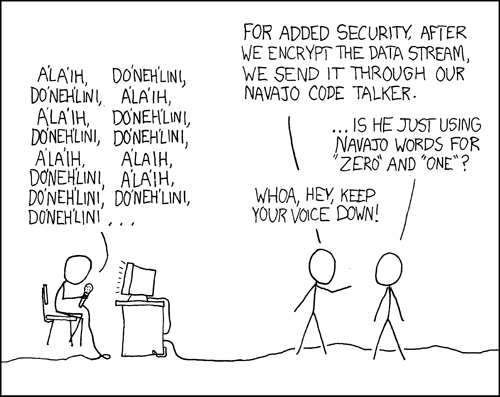
\includegraphics[width=0.75\textwidth]{Photos/Cover_page.png}}

\date{12/05/2022} % Activate to display a given date or no date (if empty),
         % otherwise the current date is printed 

\begin{document}
    
    \newpagecolor{covercolor}\afterpage{\restorepagecolor}
    \maketitle

    \parskip 0.70cm
    \newpagecolor{fadedyellow}
    
    {
        \hypersetup{linkcolor=darkBlue}
        \tableofcontents
    }

    \mychapter{0}{Author's Note}\label{chap:Auth_note}
	
	\begin{tcolorbox}[colback=MustardAddicted!5!white,colframe=MustardAddicted!75!black]
		\small Hello! \vspace{0.5cm}
		Here are a few things which I would like you, the reader, to know before you start with the report-
		\begin{itemize}
			\item This report is written as a beginner's guide to Cryptography. I have tried to ensure that the initial learning curve is gentler. In doing so, a bit of mathematical rigour and some technical aspects are glossed over. In a lot of places, informal language was also used to break up some breathing space in between all of the jargon.
			\item \cite{Silverman} was a heavy influence in writing this report. I have mostly stuck to the format of the reference textbook in the later sections of this report but if time permits, I would like to explore some more topics outside of the actual book.
			\item The colour \hyperref[chap:Auth_note]{``teal''} has exclusively been used for hyperlinks to ensure that the reader is able to read the further sections without having to skim through every concept discussed before that. (Only the table of contents has hidden hyperlinks)
			\item It is highly recommended that the reader goes through the first chapter (\emph{Mathematical Base to Cryptography}) before continuing to other sections. But it is understandable that s/he might get bored by just theoritical knowledge without seeing any link to cryptography so they can free go to any of the further sections. Wherever possible, I have added hyperlinks, in the later chapters, to the earlier concepts to ensure that the first chapter can act as a look-up table for readers.
		\end{itemize}
	\end{tcolorbox}

	\mysection{1}{Acknowledgements}
		This work was written as a part of the Summer Of Science, 2022 by the MnP Club, IIT Bombay. I read in its entirety \cite{CodeBook} to get a surface level introduction to the topic and then mostly followed the reference book \cite{Silverman} and referred to online resoruces like \cite{Hypr} for a deeper dive. \par Some of the sections in the report are heavily inspired by the above resources and at several points might simply be a paraphrasing of the reference books. Nevertheless, I have tried to compress the contents of these sources wherever needed, explored some minor topics on my own to a deeper depth, and tried my best to break down too much of difficult mathematics into easier chunks while still preserving sufficient depth. \par I would like to acknowledge the help of my mentor, Param Rathour, for his help and support. He was extremely helpful and friendly and his enthusiasm for the topic definitely rubbed off on me and gave me enough encouragement to devote the hours I have put into this report. He cleared my doubts at every stage at the latest and that allowed me to get through some of the most difficult sections of this report.\par Some topics in the end had to be skipped as they were only explored partially and so I opted to remove them completely in order not to ruin the structure of this report.\normalsize
    

\newtheorem*{remark}{}
\newtheorem*{definition}{Definition}

\mychapter{1}{Mathematical Base to Cryptography}
\begin{center}
	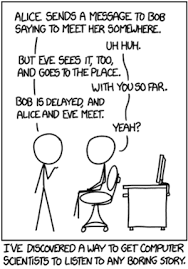
\includegraphics{Photos/chapter_cover_1.png}
\end{center}

	
	\mysection{1}{Introduction to Cryptography}

		\subsection{Some terminologies}
		\begin{itemize}
			\item \emph{Plaintext,} The message, usually alphabetic in this context, that you wish to send. \\ Depicted using small letters \(a\), \(b\), \(c\), \( \cdots \) 

			\item \emph{Ciphertext,} The message that will be transmitted after enciphering. \\ Depicted using captial letters \(A\), \(B\), \(C\), \(\cdots\)

			\item \emph{Key,} The word/ phrase/ alphabetic order using which we encrypted our \emph{Plaintext}.

			\item \emph{Monoalphabetic Substitution Cipher,} A cipher key which uses only one set of alphabet to encrypt the \emph{Plaintext}

			\item \emph{Polyalphabetic Substitution Cipher,} A key that consists of multiple alphabetic orders/  keywords to encrypt the message.  

			\item \emph{Alice, Bob and Eve,} The quintessential trio studied in Cryptology examples wherein \emph{Alice} and \emph{Bob}, are trying to communicate secretly which \emph{Eve} tries to intercept and decrypt the messages.
		\end{itemize}

	 	\subsection{Early Cryptography}
	 		The earliest forms of monoalphabetic\footnote{Consisting of only 1 key} ciphers include the \emph{Caesarean/Shift Cipher}. This involves shifting of the alphabet by a few (historically 3) letter to encrypt the \emph{Plain text.} \\
	 		This yields us with only 26 possible cipher keys which can be easily cycled through by Eve, once she is sure that Caeser Cipher has been used, hence providing us with next none security. \par
	 		Of course, there exist a very large number of random monoalphabetic cipher keys (\(26! \approx 4\times10^{26}\) to be precise) but monoalphabetic ciphers can be easily broken into using statistical analysis of the cipher text. Tools employed by cryptanalysts include- 
	 		\begin{itemize}
	 			\item Frequency of letters
	 			\item Frequency of Bigrams (pairs of letters that occur together)
	 			\item Presence of vowels 
	 		\end{itemize}
	 		\begin{mybox}Another classical cipher, which used polyalphabetic cipher keys, \emph{Vigen\`{e}re} cipher will be analysed in later weeks.\end{mybox}
	 
	 \begin{mdframed}
	 \mysection{2}{Some Mathematical Pre-requisites for Modular Arithematic}
	 	\subsection{GCD}\label{subsec:gcd}
	 		\begin{definition}\label{def:Euclid}
	 			\emph{GCD} of any 2 integers is the largest positive integer that divides each of the integers, provided both integers aren't 0.
	 		\end{definition}
	 		The standard procedure to find \(\gcd(a,b)\) is to list out factors of \(a\) and \(b\), and choose the largest factor common to both. But an even faster algorithm exists called the \emph{Euclid's algorithm}. It uses the fact that \(\gcd(a,b)=\gcd(a-k \cdot b, b), \forall a,b,k \in \mathbb{Z}\) such that \( a>b\)\footnote{Proof: Suppose you have 2 numbers \(a, b\) such that \(\gcd (a,b) = g\) thus we can write \(a = p \cdot g\) and \(b = q \cdot g\). Obviously then, if we defined \(c = a-b= (p-q) \cdot g\), will have \(g\) as a divisor. \\ Futhermore, let us denote \(\gcd(b,c)=h\). Thus we can also write \(b = m \cdot h\) and \(c = n \cdot h\). Upon rearranging, we get \(a=b+c=(m+n)\cdot h\) which tells us clearly that \(h\) will have to be a divisor of \(a\).\\ Now, at this point, all of \(a, b\) and \(c\) have both \(g\) and \(h\) as factors. So the only way \(\gcd(a,b)\) does not exceed the initially set \(g\) is because \(g = h\). \textcolor{orange}{Tada!}} \par
	 		Thus to find \(\gcd(A,B)\), we can use this algorithm
	 		\begin{enumerate}
	 			\item Take $a=A$, $b=B$
	 			\item If $b>a$, swap them.
	 			\item \(\gcd(a, b)=\gcd(a-k \cdot b, b)\) so replace \(a\) with \(a-k \cdot b\) such that \((k+1) \cdot b > a\) and \(k \cdot b < a\)
	 			\item If \(a=0\), \(\gcd(A,B)=b\) \\ else swap $a$ and $b$, and repeat from Step 3. 
	 		\end{enumerate}
	 		\textbf{Some interesting results-}
	 		\begin{itemize}
	 			\item \(r_{n+2}<\frac{r_n}{2}\) where \(r_n\) is the $n^{th}$ remainder\footnote{Proof- Assuming 2 cases (1. \(r_{n+1}<\frac{r_n}{2}\) is obvious,2. \(r_{n+1}>\frac{r_n}{2}\) ensures that \(r_n=1.r_{n+1}+r_{n+2} \Rightarrow r_{n+2}=r_n-r_{n+1}<\frac{r_n}{2}\))}.
	 			\item it takes at most \(2 \log_{2}{b} +2\) steps\footnote{We can use the fact that if \(b \in [2^{n-1}, 2^n)\) and \(r_{2k+1}<\frac{b}{2^{k}}\), we can easily see that this is true since \(2n+1=2(n-1)+2<2 \log_{2}{b} +2\) }.
	 			\item We can prove that \(\gcd(a,b)=u \cdot a + v \cdot b\) where \(u, v \in \mathbb{Z}\). These \(u, v\) values can be determined using a simple algorithm if we know the quotients at each step. \\
	 			We can even find the original \(a\) and \(b\) if we have all the quotients.
	 			\item The above statement also means that if \(\gcd(a,b)=1\), we can write any number using linear combinations of \(a\) and \(b\). 
	 		\end{itemize}
	 \end{mdframed}
	 
	 \mysection{3}{Modular Arithematic}
	 	\subsection{Format}
	 		\centering \(a \equiv b \bmod(m)\) where \(a-b\) is divisible by $m$ \par
	 		\raggedright  
	 	
	 	\subsection{Properties}
	 	\begin{itemize}
	 		\item If \(a \cdot b \equiv 1 \bmod(m)\ \exists b \in \mathbb{Z} \iff \gcd(a,m)=1\), we say that $b$ is the \emph{modular inverse} of $a$ modulo $m$. \\
	 		\emph{\underline{Note-} Although multiple values of $b$ will exist if \(\gcd(a,m)=1\), all will have the same value of \(b \bmod(m)\). Hence we used the term \textbf{the inverse}.}
	 		\item If \(a_1 \equiv b_1 \bmod(m)\) and \(a_2 \equiv b_2 \bmod(m)\), then, \(a_1 \cdot a_2 \equiv b_1 \cdot b_2 \bmod(m)\)
	 		\item We can denote \emph{inverse} of $a$ as \(a^{-1}\) such that, \(a^{-1} \equiv b \bmod(m)\). \\
	 		Hence \(7^{-1} \equiv 8 \bmod(11)\). This means if we can write \(\frac{4}{7} \equiv 7 \cdot 8 \bmod(11) \equiv 1 \bmod(11)\) as \(4 \equiv 7 \bmod(11)\). \\
	 		\emph{The interesting thing to note here is that it isn't easy to find the modular inverses of numbers as \(m\) becomes larger.}
	 		\item Since we can write \(a \cdot b \equiv 1 \bmod(m)\) as \(a \cdot b= q \cdot m + 1\), from the result obtained in last section, we can be sure that finding a value of b will take no. of steps \(\sim \log_{2}m\).
	 	\end{itemize}

	 	\begin{tcolorbox}
	 		You might think that finding the modulo of products of large numbers might take the same amount of time as it takes for calculating the product but you can easily cut down time on it. \\ Example- \(170242 \times 261494 \bmod(10) \equiv 2 \times 4 \equiv 8 \bmod(10)\). Hence it is \textcolor{red}{\textbf{\underline{\emph{FAST}}}}.
	 	\end{tcolorbox}

	 	\subsection{Ring theory}
	 		As we can see in the above definitions, it is obvious that in \(a \equiv r \bmod(m)\), \(r \in [0, m-1] \cap \mathbb{Z}\). We can then say that \(r \in \mathbb{Z}/ m \mathbb{Z}\) where \(\mathbb{Z}/ m \mathbb{Z}\) is the ring of integers with modulo \(m\). \par
	 		\indent For addition and multiplication in \(\mathbb{Z}/ m \mathbb{Z}\) space, we just divide the answer with \(m\) and use the remainder as final value.
	 		\\
	 		\noindent \emph{Units modulo m-} If \(\gcd(a,m)=1\), OR \(a^{-1}\) exists for modulo \(m\), we say that $a$ is units modulo $m$. 
	 		\begin{itemize}
	 			\item If \(a_1, a_2\) are units modulo \(m\), \( a_1 \cdot a_2 \) will also be a units modulo \(m\).
	 			\item If \(a_1, a_2\) are units modulo \(m\), \( a_1 + a_2 \) need not be a units modulo \(m\).
	 		\end{itemize}
	 		The set \(\ast(\mathbb{Z}/ m \mathbb{Z})\) is called the group of units modulo \(m\) and can also be defined as-
	 		\centering \(\ast(\mathbb{Z}/ m \mathbb{Z})={a\in \mathbb{Z}/ m \mathbb{Z}, \gcd(a,m)=1}\)
	 		\raggedright If we took a subset of units modulo \(m= \textbf{P}\), then-
	 		\begin{itemize}
	 			\item If \(k_{i,j}= a_i \cdot a_j,\) where \(a_i, a_j \in \textbf{P},\) then \(k_{i,j}\) also belongs to \(\textbf{P}\).
	 			\item If \(k_{i,j}= a_i + a_j,\) where \(a_i, a_j \in \textbf{P},\) then \(k_{i,j}\) need not belong to \(\textbf{P}\).
	 		\end{itemize}
	 		\textbf{Euler's Totient/ Phi Function-} \(\phi(m)=\# \ast(\mathbb{Z}/ m \mathbb{Z})\) OR $\phi(m)$ counts the number of \(a \in [1,m-1]\), such that, \(\gcd(a,m)=1\) i.e. number of values of \(a<m\) such that \(a\) and \(m\) are co-prime\\
	 		\emph{e.g. \(\phi(24)=8, \phi(7)=6\)} \\ \emph{\underline{Note-} Notice how \(\phi(p)\) where \(p\) is a prime number, will always be \(p-1\)}

	 	\subsection{Shift Ciphers and Modulo Arithematic}
	 		We can assign numbers from 0 through 25 to all the letters in the alphabet and then use modulo arithematic for encryption and decryption-
	 		\begin{itemize}
	 			\item For a shift of \(k\), we can encrypt any letter whose number is denotes by \(p\) to a letter \((p+k) \bmod(26)\)
	 			\item To decrypt the cipher text (\(p'\)), you subtract in the ring via \((p'-k) \bmod(26)\).
	 		\end{itemize}
	 	\subsection{Fast Powering algorithm}\label{subsec:fastexpo}
	 		To calculate \(g^A \bmod(m)\), where \(g, A \in \mathbb{N}\), it can take \(\sim 2^n)\) multiplications if \(A \in [2^n, 2^{(n+1)})\). We can, however, use the fact that $g$ can we written as a linear combination of powers of 2 to reduce the number of steps we take.
	 		\begin{itemize}
	 			\item Express \(A=\sum_{n=0}^{k}{a_r 2^r}\) where \(2^k \leq A < 2^{(k+1)}\)
	 			\item Let \(g_r = g^{2^r}\). We can find \(g_1\) using \(g \cdot g\) and for subsequent values of r, we can just use \(g_{r+1} = g_r \cdot g_r\)
	 			\item Now we have \(g^A = 
	 			\sum_{r=0}^{k}{g^{a_0 + a_1 \cdot 2 + a_2 \cdot 2^2 +\cdots}}=
	 			\sum_{r=0}^{k}{g_0^{a_0}+ g_1^{a_1} + \cdots}\)
	 			\item \(x^2 \bmod(N) = (x \bmod(N))^2 \bmod(N)\)
	 		\end{itemize}
	 		Keep in mind that \(a_r\) can only take the values 0 and 1 thus we can say that this method takes \(2r\) multiplication steps at most. (Including the exponential expansion of \(A\)).
	 \mysection{4}{Prime numbers and Finite Fields}\label{sec:prime}
	 	\subsection{Division modulo $m$}
	 		We can usually do multiplication, subtraction, addition modulo \(m\) but division modulo \(m\) is only possible if the divisior(\(k\)) is coprime with \(m\). \par
	 		\noindent \emph{Divison modulo \(m\) means- If \(a=p\bmod(m)\) and \(b=q \bmod(m)\),} \par
	 		\centering\emph{\(c= \frac{a}{b}= \frac{p'}{q'}\)} \par
	 		\raggedright where \(p \bmod(m) = p' \bmod(m)\) and \(q \bmod(m) = q' \bmod(m)\) and \(\frac{p'}{q'} \in \mathbb{Z}\). It is only possible if \(\gcd(b,m)=1\) as otherwise you cannot get a unique value. \\
	 		Example- \(a= 11 \bmod (5)\), \(b = 4 \bmod (5)\) then \(\frac{a}{b}= \frac{11 \bmod (5)}{4 \bmod (5)}=\frac{16 \bmod (5)}{4 \bmod (5)}\)=4\\
	 		\emph{Note-} In the above example, 4 is the only integral value possible of \(\frac{a}{b}\). Values such as \(\frac{11 \bmod(5)}{4 \bmod(5)}=\frac{1}{4}\) are ignored. \par

	 		The reason for \(\gcd(4, 5)=1\) being necessary in the above examples is that we can write \(\frac{11 \bmod(5)}{4 \bmod(5)}= 11 \cdot 4^{-1} \bmod(5)\) and \(4^{-1}\) can only exist if \(\gcd(4,5)=1\). (Here \(4^{-1}= 4\) thus our answer = \(44 \bmod (5)=4\))

	 	\subsection{Division in rings}
	 		As seen earlier, if \(\gcd(a,m)=1\), we can easily divide modulo \(m\) by a any integer. If we now studied rings of form \(\mathbb{Z}/p\mathbb{Z}\), where \(p \in prime\) we will get that any integer \(b\in \mathbb{Z}/p\mathbb{Z}\) can be used in division as obviously \(b<p\) AND \(p\in prime\) thus \(\gcd(b,p)=1\) \par
	 		
	 		\begin{mybox}\label{theo:extendedEuclid}
	 			\underline{Note-} If \(a\in\ast\mathbb{Z}/m\mathbb{Z}\), \(a\) can be used as a divisor modulo $m$. ALSO \(\mathbb{Z}/p\mathbb{Z}\)= \(\ast \mathbb{Z}/p\mathbb{Z}\). \par
	 			\emph{We can calculate \(a^{-1}\) using- \(au+pv=1\) (as \(\gcd(a,p)=1\)), wherein solving for $u$ yields us \(a^{-1} \bmod(p)\).}
	 			\tcblower
	 			The last line is the \textbf{Extended Euclidean Theorem}. Unlike the normal \hyperref[def:Euclid]{Euclid's theorem}, the easiest way to describe its working is via a \hyperref[add:codeForRecursive]{recursive C code}.
	 		\end{mybox}

	 	\subsection{Finite Fields}
	 		Since we can compute division, addition, multiplication and subtraction in \(\mathbb{Z}/p\mathbb{Z}\), we can call it a field just like \(\mathbb{R}/\mathbb{Z}/\) etc\(\cdots\) \\
	 		Since \(\mathbb{Z}/p\mathbb{Z}\) only has a finite number of elements, we call it a finite field and can even denote it by \(\mathbb(F)_p\) to show the finitedness.
	 \mysection{5}{Fermat's ``Little'' Theorem}\label{sec:fermat}
	 	The theorem states that- \par
	 	\centering \(a^{p-1} \equiv 1 \bmod(p)\) for \(a \not = k \cdot p\) \par
	 	\begin{mdframed}
		 	\raggedright \textbf{Proof:} \\
		 	Since \(a \not= k \cdot p\), \(a, 2a, 3a, 4a, \cdots (p-1)a \bmod(p) \not= 0\). Now if we considered \(k \in [1,p-1]\), \par
		 	\centering \(k_1 \cdot a \equiv j_1 \bmod(p)\) AND \(k_2 \cdot a \equiv j_2 \bmod(p)\) \par
		 	\(\Rightarrow (k_1-k_2)\cdot a \equiv (j_1-j_2) \bmod(p)\) \par
		 	\raggedright Since \(k_1 - k_2\) cannot be a multiple of \(p\), \(j_1 - j_2 \not= 0\) and so for every \(k \in [1, p-1]\), we get a distinct \(j \in [1, p-1]\). Hence we get a bijective function of \([1,p-1] \rightarrow [1,p-1]\). So- \par
		 	\centering \( \prod_{k=1}^{p-1}k \cdot a \equiv  \prod_{k=1}^{p-1}{k} \bmod(p) \Rightarrow (p-1)! a^{p-1} \equiv (p-1)! \bmod(p)\) \par
		 	\(\Rightarrow a^{p-1}=1 \bmod(p)\)
	 	\end{mdframed}
	 	\raggedright We can use this to find the inverse of any number modulo \(p\)- \\ \centering \(a\cdot a^{p-2}\equiv 1 \bmod(p) \Rightarrow a^{-1} \equiv a^{p-2} \bmod(p)\) \par \par  
	 	\LARGE \emph{\textcolor{orange}{Voila!}}  \\ \tiny We just found an inutitive, new way to check if a number is composite or not \par
	 	\raggedright \small If we wanted to check if a number \(n\) was prime or not-
	 	\begin{itemize}
	 		\item If \(n \in even\), obviously composite
	 		\item If \(n\in odd\), take \(a=2\). Now if \(2^{n-1} \not \equiv 1 \bmod(n)\), we can be sure that it is definitely composite. \footnote{As is with all good things in life, this too has an asterisk- you cannot judge if a number is prime or not solely based on this. There is a subset of composite numbers called the ``Carmicheal Numbers'' which satisfy \(b^{(n-1)} \equiv 1 \bmod(n)\) despite their lack of primality. Just random gifts of joy Mathematics bestows upon you. It is better discussed in \hyperref[subsec:witness]{a later section}.} \\
	 	\end{itemize}
	 	\definition{\emph{We define} order \emph{as the smallest number \(k\) such that}} \par 
	 	\centering \(a^k\equiv 1 \bmod(p)\) \par 
	 	\raggedright \em We can also be sure that \(p-1\) is divisible by \(k\). 
		 \subsection{Primitive Roots Theorem}\label{subsec:primitive}
		 The theorem states that \emph{for a prime number $p$, there always exists a number \(g \in \mathbb{F}_p\), such that every element of \(\mathbb{F}_p^{*}\) can be expressed as a power of $g$ } \par
		 Number of primitive roots of \(p= \phi(p-1)\)
		 \begin{tcolorbox}
		 	\textbf{Example-} Let us study \(\mathbb{F}_7^*\). Since \(7 \in \text{primes}\), \(\mathbb{F}_7^* \equiv \mathbb{F}_7\). \\
		 	3 is considered a primitive root of this finite field so-
		 	\[1, 3, 3^2, 3^3, 3^4, 3^5, 3^6 \bmod(7) \equiv 1, 3, 2, 6, 4, 5, 1\]
		 	Even 5 is considered as so-
		 	\[1,5,5^2,5^3,5^4,5^5,5^6 \bmod(7)\equiv 1,5,4, 6, 2, 3, 1\]
		 	However 6 is not one-\label{example:six}
		 	\[1,6,6^2,6^3,6^4,6^5,6^6 \bmod(7) \equiv 1, 6, 1, 6, 1, 6,1\]
		 	(Note how despite 6 despite not being a primitive root, still satisfies \(6^{p-1} \bmod(p) \equiv 1\).)\\

		 	\(\phi(6)=\phi(2\times3)=1\times 2=2\) thus number of primitive roots of \(7 \equiv \phi(7-1) = 2\) 
		 \end{tcolorbox}

	\mysection{6}{Symmetric Ciphers}
		\subsection{Notations}
			If you have a message \(m \in \mathcal{M} \) (where \(\mathcal{M}\) is the list of all possible messages), you can choose a key \(k \in \mathcal{K}\) (again, where \(\mathcal{K}\) is the space of all keys), to get a cipher \(c \in \mathcal{C}\). (At this point if you cannot guess what \(\mathcal{C}\) stands for, I don't think you should read further).\par
			We thus need invertible functions \(e_k(m)\) and \(d_k(m)\) as -\par
			\centering \(e_k(m_i)= c_i\) AND \(d_k(e_k(m))=m\) \par
			\raggedright

		\subsection{Principles of Succesful Ciphers}
			\begin{mybox}
				Kerckhoff’s principle says that the security of a cryptosystem should depend only on the secrecy of the key, and not on the secrecy of the encryption algorithm itself. 
			\end{mybox}
			So keeping that in mind, we design a few principles-
			\begin{enumerate}
				\item For any plaintext \(m\) and key \(k\), it must be easy to calculate \(e_k(m)\).
				\item For any ciphertext \(c\) and key \(k\), it must be easy to calculate \(d_k(m)\).
				\item If you have ciphertexts \(c_1, c_2, c_3\cdots c_\alpha\) encrypted using the key \(k\), it should be really difficult to find \(d_k(c_1), d_k(c_2), \cdots d_k(c_\alpha)\) without knowing \(k\).
				\item If you have \(c_1, c_2, c_3, \cdots c_\beta\) and the corresponding messages \(m_1, m_2, m_3, \ldots m_\beta \), it should still be difficult to decipher a \(c\) not in this set.
			\end{enumerate}

		\subsection{Encoding of Cipher Blocks}
			We can represent any plaintext in the form of bits \(m_{B-1}m_{B-2}\cdots m_2m_1m_0\) where \(m_i \in {0,1} \forall i\in [0,B)\). Then we can break it into bytes or blocks of some other size and encode each block separately. We prefer to choose a \(\mathcal{K}\) such that \(k \in [0, 2^{B_k})\) and \(B_k \geq 80\) bits or \(160\) bits based on the message type. (This number is chosen based on the computing capacity of a modern computer since you can brute-force check each and every key \(k \in \mathcal{K}\), if \(B_k\) is not large enough.) 

		\subsection{Examples of Symmetric Ciphers}
			Choose \(\mathcal{K}=\mathcal{C}=\mathcal{M}=\mathbb{F}_p^*\) for some prime number \(p\) and then you can define- \par
			\centering \(e_k(m)\equiv k \cdot m \bmod(p)\) \par
			\raggedright Using that you can also find \(k'\) (in \(2\log_2(p)+ 2\) steps) such that- \par
			\centering \(d_k(c)\equiv k' \cdot c \bmod(p)\) to yield us \(d_k(c) \equiv m\) \par
			\raggedright Although this method follows the first 3 principles, it fails the fourth principle of successful ciphering as- \par
			\centering \(k \equiv m^{-1} \cdot c \bmod(p)\) \par 
			\raggedright The above formula gives you the exact key as soon as you find one pair of ciphertext and plaintext thus is not preferable at all.

			\subsubsection*{Simple multiplicative cipher}
				If instead of using a modulo p, if you just used \(e_k(m)= k \cdot m\), you can easily find \(\gcd(c_1, c_2, c_3 \cdots c_\alpha)\) which can give you the value of \(k\) outright. (Calculating GCD of multiple numbers is not labour intensive for a computer)

			\subsubsection*{Affine Cipher}
				Here we define ciphertext using both multiplication and addition modulo p- \par
				\[e_k \equiv k_1 \cdot m + k_2 \bmod(p)\] AND \[d_k(c) \equiv k_1' \cdot (c-k_2) \bmod(p)\] \par	
				\raggedright \emph{Note- Caesarean Shift Cipher is just a special case of this cipher with \(k_1 = 1\)} \par 

			\subsubsection*{Hill Cipher}
				In this cipher, we first denote every message of length \(n\) as a \(n \times 1\) column matrix. Then we can define a key \(k= k_{1,1}k_{1,2}k_{1,3}\cdots k_{n,n}\) as- \par 
				\[
				k=
				\begin{bmatrix}
					k_{1,1} & k_{1,2} & k_{1,3} & \dots & k_{1,n}\\
					k_{2,1} & k_{2,2} & k_{2,3} & \dots & k_{1,n}\\
					k_{3,1} & k_{3,2} & k_{3,3} & \dots & k_{1,n}\\
					\vdots & \vdots & \vdots & \ddots & \vdots \\
					k_{n,1} & k_{n,2} & k_{n,3} & \dots & k_{n,n}
				\end{bmatrix}
				\]
				We can calculate the inverse of \(k= k^{-1}\) and using the both of them, our cipher looks like-
				\[
				\begin{bmatrix}
					k_{1,1} & k_{1,2} & k_{1,3} & \dots & k_{1,n}\\
					k_{2,1} & k_{2,2} & k_{2,3} & \dots & k_{1,n}\\
					k_{3,1} & k_{3,2} & k_{3,3} & \dots & k_{1,n}\\
					\vdots & \vdots & \vdots & \ddots & \vdots \\
					k_{n,1} & k_{n,2} & k_{n,3} & \dots & k_{n,n}
				\end{bmatrix}
				\cdot 
				\begin{bmatrix}
					m_{1,1}\\
					m_{2,1}\\
					m_{3,1}\\
					\vdots \\
					m_{n,1}
				\end{bmatrix}
				=
				\begin{bmatrix}
					c_{1,1}\\
					c_{2,1}\\
					c_{3,1}\\
					\vdots \\
					c_{n,1}
				\end{bmatrix}
				\]
				Unfortunately both Affine and Hill Ciphers are both susceptible to plain text attacks. Hence we cannot use either one of these despite how dapper they look.

			\subsubsection*{XOR Cipher}
				XOR \(\oplus\) of key and message \(c \equiv m \oplus k\) seems like a good option but it has the following flaw if you have access to 2 ciphers made using the same key-
				\[
					c' \oplus c \equiv (m' \oplus k) \oplus (m \oplus k) \equiv m' \oplus m
				\]
				\begin{center}
				\begin{tabular}{c | c  c}
					 \(m\oplus m'\)&Possible $m$ &Possible $m'$\\ 
					 \hline
					 0&0&0\\
					 0&1&1\\
					 \hline
					 1&0&1\\
					 1&1&0\\
					 \hline  
				\end{tabular}
				\end{center}
				Thus we can easily find information about \(m\) from just 2 ciphers. (Although still \(m\) exactly isn't visible)

		\subsection{Random bit sequences}\label{subsec:random}
				To circumvent the above issue, we can use different ``keys'' for different messages that we encrypt. One way to do that is to use a key \(k\) and a pseudo-random\footnote{Not called ``random'' as we are using some algorithm to generate it after all.} number generator \(\mathcal{R}\) such that-
				\[
					\mathcal{R} : \mathcal{K} \times \mathbb{Z} \rightarrow {0,1}
				\]
				Thus we can use this to construct a sequence of n-bits (the XOR key) \(j_1j_2j_3 \cdots j_n\) such that \(j_i = \mathcal{R}(k, i)\) if message to be encrypted has n bits as well. Then we can just sequentially go through every bit of the message and apply \(\oplus\) with bits of the XOR key.
	\mysection{7}{Asymmetric Ciphers}\label{sec:asym}
		One flaw with symmetric ciphers is that the key used for encryption is same as the one used for decryption. Hence for \emph{Alice} to send a message to \emph{Bob}, she has to first send him a copy of the key she used for encryption. However, in the information age, that key is equally susceptible to being intercepted by \emph{Eve} hence undermining the privacy of \emph{Alice} and \emph{Bob}.\par
		One effective way to combat this is having a public key used for encryption (\(k_{public}\)) and a {private} key for decryption (\(k_{private}\)). As the names suggest, the former is available freely and can be used by anyone while sending information to \emph{Alice} but only \emph{Alice} has the latter key. \\
		Some important details of this method-
		\begin{itemize}
			\item \(e_{k_{public}}(m_i) = c_i\) and \(d_{k_{private}}(c_i)=d_{k_{private}}(e_{k_{public}}(m_i))=m_i\).
			\item It should be infeasible to calculate \(k_{private}\) using just knowledge of \(k_{public}\).
		\end{itemize}




    
	\mysection{8}{Probability Theory}
		\subsection{Basics}
			Well the basics are luckily... pretty basic. All of the stuff we learnt already in JEE. Some of the interesting concepts are in the next few sections.

		\subsection{Monty Hall Problem}
		\begin{greenbox}
			\centering \emph{Suppose you’re on a game show, and you’re given the choice of three doors: Behind one door is a car; behind the others, goats. You pick a door, say No. 1, and the host, who knows what’s behind the doors, opens another door, say No. 3, which has a goat. He then says to you, “Do you want to pick door No. 2?” Is it to your advantage to switch your choice? } \par
		\end{greenbox}

			\raggedright One important thing to keep in mind which makes the final solution seem non-intuitive \(\rightarrow\) The host knows which door has the Car behind it. He will never open the door with the car.
			Let us try to rationalise the problem based on Bayes' Theorem.\\
			Assume for now that whatever door we choose is called $Door_1$, the host opens either $Door_2$ or $Door_3$ \par

			Case 1: $Car \rightarrow Door_1$\\
			\quad In that case $P(keep\rightarrow Car)=1$ and $P(swap\rightarrow Car)=0$

			Case 2: $Car \rightarrow Door_2$\\
			\quad In that case $P(keep\rightarrow Car)=0$ and $P(swap\rightarrow Car)=1$

			Case 3: $Car \rightarrow Door_3$\\
			\quad In that case $P(keep\rightarrow Car)=0$ and $P(swap\rightarrow Car)=1$\par 

			Using Total probability theorem, it is obvious that $P(keep \rightarrow Car)= \frac{1}{3}$ and $P(swap \rightarrow Car)= \frac{2}{3}$
    \mychapter{2}{Randomness and Obfuscation}
\begin{center}
	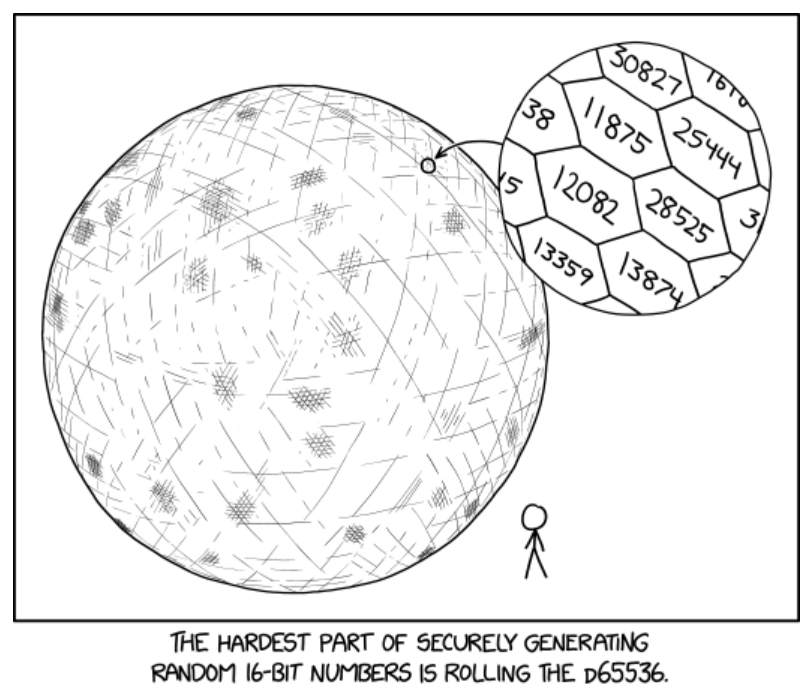
\includegraphics[width=0.75\textwidth]{Photos/random.png}
\end{center}
	\mysection{1}{Random Numbers}
		\subsection{Why do we need random numbers}
			A lot of the encryption techniques used in the later weeks will require some randomness to increase the strength of the cipher. We had already covered their importance in general in \textcolor{teal}{\hyperref[subsec:random]{Random Bit Sequences}} but in specific-
			\begin{itemize}
				\item RSA cryptosystems, despite being completely deterministic, requires some randomness in the plaintext for better security.
				\item Public key cryptosystems depend almost completely on the using random prime numbers to design the keys.
				\item Probabilistic Encryption systems definitely require incorporation of randomness into the encryption process.
			\end{itemize}

		\subsection{Is it even possible to construct an actually random number?}
			Quantum Theory states that the decay of specific atom is completely probabilistic. We can be sure that for a radioactive atom, there is a T time such that after T seconds, a undecayed atom has a \emph{50\%} chance of decaying but we cannot say with 100\% surety if a particular atom will decay or not.\par
			Thus to construct the first bit of a random number, we just study a radioactive atom for T seconds and if it decays, $bit = 1$ else $bit = 0$. \par
			Unfortunately, this is a very impractical way to construct a large random string daily use. Hence we go for pseudo random bit generators.

		\subsection{Pseudo-Random Number Generator}\label{subsec:prng}
			PRNG is just a function that takes in an initial seed \emph{S} which is truly random to algorithmically create a pseudo-random number\footnote{Called so because of the irony of having a well defined function that can create supposedly random numbers.}.\par
			The two properties that a PRNG should have for it to be considered cryptographically secure are-
			\begin{enumerate}
				\item If \emph{Eve} has the first \emph{k} bits of the PRN, she should not be able to predict the next bit with a more than 50\% chance.
				\item If \emph{Eve} has some the bits in the PRN such as \(R_t, R_{t+1}, R_{t+2} \cdots\), she should not be able to predict any of \(R_1, R_2, \cdots , R_{T-1}\) bits with a more than 50\% surety.
			\end{enumerate}

			To continue further, some knowledge of Hash Functions is necessary.

\begin{mdframed}
	\mysection{2}{Hash Functions}
		\centering \emph{Hash Algorithmns are like a summary of the original document. It is difficult to figure out the original document from the hash output but it acts as a signature that ensures accuracy. Due to the pigeonhole problem, it is obvious that Hash collisions would occur- but a good algorithm ensures that those are incredibly difficult to happen by happenstance and equally so to artificially bring about \\ \raggedleft{- Tom Scott}}\par
		
		\raggedright Hash functions take in arbitrarily long documents \(D\) and output a shorter bit strong \(H\). Their main objective is for authentication purposes. Some important characteristics are-
		\begin{itemize}
			\item Computation of $Hash(D)$ should be fast \(\rightarrow\) \emph{linear time}
			\item Inversion of Hash(D) should be difficult \(\rightarrow \) \emph{exponential time} i.e. finding \textbf{any} \emph{D} given a hash output \(H\) of the form \(Hash(D) = H\)
			\item Ideally we want Hash functions to have collision resistance i.e. it should be difficult for 2 non-identical documents \(D1\) and \(D2\) to give the \(Hash(D1)= Hash(D2)\). This property is important for the sake of unambiguity in differentiating between 2 possible inputs when the inteded recepient receives the Hash output.
		\end{itemize}
		\textbf{Note-} \\
		\quad a. There is a considerable difference between Authentication/ Verification and Inversion. Hash functions need to be easy to compute as well as verify but should be resistant from inversion. \\
		\quad b. Hash is not an encryption- it cannot (ideally) be decrypted back to the original message. It is just a signature.\\
		\quad c. Hash outputs are ``seemingly'' random so even a small flipping of bits in the input should completely change the hash. \par

		We ideally would base Hash functions on mathematically difficult problems to solve such as the Discrete Logaritms and Prime Factoring to ensure that inversion is difficult but that is impractical for even the encryption speeds today's world needs. So we prefer ad-hoc mixing methods such as the \emph{Secure Hash Algorithm} {SHA (or SHA-1)}  which is the universally used algorithm. 
		\subsection{How does SHA-1 work?}
		SHA outputs 160 bits no matter what you input in; if the input is a multiple of 160 bits, we just xor the first result of the \(k\)th output with the transformation of the (\(k+1\))th mixing to get the \(k+1\)th output. If the file isn't a multiple or is smaller than 160 bits, we just append 0s till we get a proper multiple. 
			\begin{enumerate}
				\item Choose 5 32-bit numbers \(h_0, h_1, h_2, \ldots, h_4\) randomly.
				\item Divide the file into chunks of 512 bits and then redivide those chunks individually into 16 blocks of 32-bits (or words) \(w_0, w_1, w_2\ldots w_15\).
				\item ``Rotate'' the words (i.e. shift the bits circularly arbitrarily \textbf{between} the words\footnote{Essentially if you have 1000, 1101, 0111, 1010 and you decided to rotate the 3rd bit in each 4-bit number, you can get a 1000, 1111, 0111, 1000 i.e. the 3rd bit of each number is extracted to form the array {0,0,1,1} and this is rotated as the algorithm is designed} (not inside the words individually)) to create 80 words \(w_0, w_1, w_2, \ldots, w_{79}\).
				\item Start the loop with i as control variable incrementing from 0 to 79. 
				\item Now just create temporarily variables \(a=h_0\), \(b=h_1, \; \ldots e=h_4\) and construct \(f\) from some arbitrary combination of \(a, b, c, d, e\) using AND and XOR.
				\item Arbitrarily mix \(a, b, c, d, e\) using some rotations, shifts and whatever you feel like adding on a lazy Wednesday afternoon.
				\item Add f and \(w_i\) to a and then equate \(h_0=h_0+a, h_1=h_1+b, \ldots ,h_4=h_4+e\).
				\item End the loop once you reach i=79. (i.e. complete 80 rounds)
				\item Do the same for all chunks just making sure that the values of \(h_0, h_1\ldots h_4\) are carried forward after each chunk.
				\item Concatenate \(h_0, h_1\ldots h_4\) to get the final 160-bit hash.
			\end{enumerate}
\end{mdframed}
			
			Thus now to create a pseudo-random number \(R_i\), we just select a specific \(Hash\) function and input into it \(S\) (A truly random number) concatenated with \(i\) to get-\[Hash(i\;||\;S)=R_i\] 

	\mysection{3}{Public Standard for making PRNGs}
		Start of with a random seed \(S\) and a key \(k\) for the cryptosystem. Let \(E_k\) be the encryption function associated with that \(k\). \\
		Every time a random number is required, create a \(D\) from some CPU parameters (temperauture and/or date and time and/or cpu usage) to get- \[C=E_k(D)\]
		Thus your random number \(R\) will be- \[R=E_k(C\; \text{xor}\; S)\]
		You can then update \(S\) to - \[S=E_k(R \;\text{xor}\; C)\]

	\mysection{4}{Stream Ciphers}
		\emph{This is an encryption technique which heavily depends on the PRNGs we defined above.}\\
		If you wanted to encrypt a 10-bit plaintext using Stream Ciphers, you will require a 10-bit keystream as well. If \(k_i\) is the \(i\)th bit of the keystream and \(m_i\) is the \(i\)th bit of the plaintext, \[c_i \equiv k_i \oplus m_i\] This keystream should be as random as possible to prevent codebreakers from predicting properties about the keystream thus getting information about the plaintext. \par
		But it is infeasible to make \(n\)-bit keystreams for large values of \(n\) hence we use PRNGs. We can thus have a \(k\) bit purely random seed \(S\) with which we can create \(R_1, R_2, R_3 \ldots, R_n\) using the above given algorithm. (Initial seed \(S\) is updated after every use as was defined in the last section to strengthen the security of the system)\par
		
		\begin{tcolorbox}\label{box:onetimepad}
			\textbf{BTW} the keystream used with Stream Ciphers is known as \emph{One Time Pad}. A \emph{n}-bit ciphertext made from a truly random \emph{n}-bit one time pad is mathematically impossible to decipher.
		\end{tcolorbox}
		
		\subsection{Deciphering Stream Ciphers}
			xor ($\oplus$) has an interesting property \(\rightarrow\)
			\begin{center}
			\begin{tabular}{ c | c | c | c}
				 $A$ & $B$ & $A \oplus B$ & $(A \oplus B) \oplus B$\\ 
				 \hline
				 0 & 0 & 0 & 0\\  
				 0 & 1 & 1 & 0\\
				 1 & 0 & 1 & 1\\
				 1 & 1 & 0 & 1   
			\end{tabular}
			\end{center}
			Hence we can say with surety that-
			\[k_i \oplus c_i \equiv k_i \oplus (k_i \oplus m_i) \equiv m_i\]
			Giving us a clear cut way to use this private key symmetric encryption system.\par
			\textbf{ALSO} since the generation of \(R_n\) does not require any subsequent \(R_{k>n}\), we can process each bit as it the CPU reads it instead of having to store it
	\mysection{5}{Block Cipher}
		Unlike Stream Cipher, Block Cipher is a lot simpler and less secure. It divides the input into chunks of bits and evaluates them separately.\footnote{A lot of these concepts and pictures are sourced from ``https://www.hypr.com/black-cipher/''} 

		\subsection{Electronic Code Book Method}
			Essentially if you have a \(k\) bit codebook and a \(n\) bit plain text, you divide the plain text into chunks of \(k\) bits (some padding scheme is employed in case \(n\;\% \;k \not = 0\)). Then you go through each chunk and find the corresponding ciphertext in the ECB (Electronic Code Book). Thus you encrypt the entire file.
			\begin{center}
			\begin{tabular}{ c | c }
				 $Plaintext$ & $Ciphertext$ \\ 
				 \hline
				 00 & 11\\   
				 01 & 01\\
				 10 & 00\\
				 11 & 10    
			\end{tabular}
			\end{center}
			\centering\emph{{2-bit Electronic Code Book}}

			\begin{mybox}
				\raggedright \LARGE{\textbf{Some minor itty bitty issues}}- \normalsize It preserves large scale structures hence it is completely useless to the most degree in obfuscating files with a large size if there is a lot of repetition.
			\end{mybox}

			Imagine a $10\times10$ picture where the brightness of each pixel is defined by a 2-bit digit
			\begin{center}
			\begin{tabular}{ c | c }
				 $Plaintext$ & $Ciphertext$ \\ 
				 \hline
				 0000 & 1001\\  
				 0001 & 1000\\
				 0010 & 0100\\
				 0011 & 0101\\
				 0100 & 0011\\
				 0101 & 0111\\
				 0110 & 1101\\
				 0111 & 1111\\
				 1000 & 0110\\  
				 1001 & 1011\\
				 1010 & 0001\\
				 1011 & 1100\\
				 1100 & 0010\\
				 1101 & 1100\\
				 1110 & 1010\\
				 1111 & 0000
			\end{tabular}
			\end{center}
			\centering\emph{{4-bit Electronic Code Book}}

			\[
				\begin{bmatrix}
					\color{red}00 & \color{red}00 & \color{red}00 & \color{red}00 & \color{red}00 & \color{red}00 & \color{red}00 & \color{red}00 & \color{red}00 & \color{red}00\\
					\color{red}00 & \color{red}00 & \color{red}00 & \color{red}00 & \color{red}00 & \color{red}00 & \color{red}00 & \color{red}00 & \color{red}00 & \color{red}00\\
					\color{red}00 & \color{red}00 & \color{blue}01 & \color{blue}01 & \color{blue}01 & \color{blue}01 & \color{blue}01 & \color{blue}01 & \color{red}00 & \color{red}00\\
					\color{red}00 & \color{red}00 & \color{blue}01 & \color{yellow}\color{yellow}10 & \color{yellow}10 & \color{yellow}10 & \color{yellow}\color{yellow}10 & \color{blue}01 & \color{red}00 & \color{red}00\\
					\color{red}00 & \color{red}00 & \color{blue}01 & \color{yellow}10 & \color{green}11 & \color{green}11 & \color{yellow}10 & \color{blue}01 & \color{red}00 & \color{red}00\\
					\color{red}00 & \color{red}00 & \color{blue}01 & \color{yellow}10 & \color{green}11 & \color{green}11 & \color{yellow}10 & \color{blue}01 & \color{red}00 & \color{red}00\\
					\color{red}00 & \color{red}00 & \color{blue}01 & \color{yellow}\color{yellow}10 & \color{yellow}10 & \color{yellow}10 & \color{yellow}\color{yellow}10 & \color{blue}01 & \color{red}00 & \color{red}00\\
					\color{red}00 & \color{red}00 & \color{blue}01 & \color{blue}01 & \color{blue}01 & \color{blue}01 & \color{blue}01 & \color{blue}01 & \color{red}00 & \color{red}00\\
					\color{red}00 & \color{red}00 & \color{red}00 & \color{red}00 & \color{red}00 & \color{red}00 & \color{red}00 & \color{red}00 & \color{red}00 & \color{red}00\\
					\color{red}00 & \color{red}00 & \color{red}00 & \color{red}00 & \color{red}00 & \color{red}00 & \color{red}00 & \color{red}00 & \color{red}00 & \color{red}00\\
				\end{bmatrix}
				\ch{->[ECB]}
				\begin{bmatrix}
					\color{red}10 & \color{red}01 & \color{red}10 & \color{red}01 & \color{red}10 & \color{red}01 & \color{red}10 & \color{red}01 & \color{red}10 & \color{red}01\\
					\color{red}10 & \color{red}01 & \color{red}10 & \color{red}01 & \color{red}10 & \color{red}01 & \color{red}10 & \color{red}01 & \color{red}10 & \color{red}01\\
					\color{red}10 & \color{red}01 & \color{blue}01 & \color{blue}11 & \color{blue}01 & \color{blue}11 & \color{blue}01 & \color{blue}11 & \color{red}10 & \color{red}01\\
					\color{red}10 & \color{red}01 & \color{orange}11 & \color{orange}01 & \color{pink}00 & \color{pink}01 & \color{brown}10 & \color{brown}11 & \color{red}10 & \color{red}01\\
					\color{red}10 & \color{red}01 & \color{orange}11 & \color{orange}01 & \color{green}00 & \color{green}00 & \color{brown}10 & \color{brown}11 & \color{red}10 & \color{red}01\\
					\color{red}10 & \color{red}01 & \color{orange}11 & \color{orange}01 & \color{green}00 & \color{green}00 & \color{brown}10 & \color{brown}11 & \color{red}10 & \color{red}01\\
					\color{red}10 & \color{red}01 & \color{orange}11 & \color{orange}01 & \color{pink}00 & \color{pink}01 & \color{brown}10 & \color{brown}11 & \color{red}10 & \color{red}01\\
					\color{red}10 & \color{red}01 & \color{blue}01 & \color{blue}11 & \color{blue}01 & \color{blue}11 & \color{blue}01 & \color{blue}11 & \color{red}10 & \color{red}01\\
					\color{red}10 & \color{red}01 & \color{red}10 & \color{red}01 & \color{red}10 & \color{red}01 & \color{red}10 & \color{red}01 & \color{red}10 & \color{red}01\\
					\color{red}10 & \color{red}01 & \color{red}10 & \color{red}01 & \color{red}10 & \color{red}01 & \color{red}10 & \color{red}01 & \color{red}10 & \color{red}01\\
				\end{bmatrix}
			\]
			\raggedright In the above illustration, despite the codebook using more bits than the individual pixels in the image, it still cannot obfuscate efficiently the initial file hence giving a lot of information away like-
			\begin{enumerate}
				\item The length of the codebook string.
				\item Presence of repeated structures such as the brightspot in the middle and the darkspace in the periphery.
				\item General lack of self respect for having used such a unsophisticated method.
			\end{enumerate}

			We can clearly see the issue here- inability of the encryption system to convert the same number to 2 different numbers if they occur at 2 different places. Hence we use \emph{Cipher Block Chaining (CBC)}.

		\subsection{Cipher Block Chaining}
		In this encryption method, the outcome of the previous encryption decides the outcome of the next encryption. Just like ECB mode, we do have a codebook we refer to for each chunk.
		\begin{SCfigure}[0.5][h]
			\caption{We can clearly see that the first IV (intialisation vector) is xor-ed with the first chunk. The cipher text of the first chunk is then used similarly. Notice how repeated structures are not visible anymore.}
			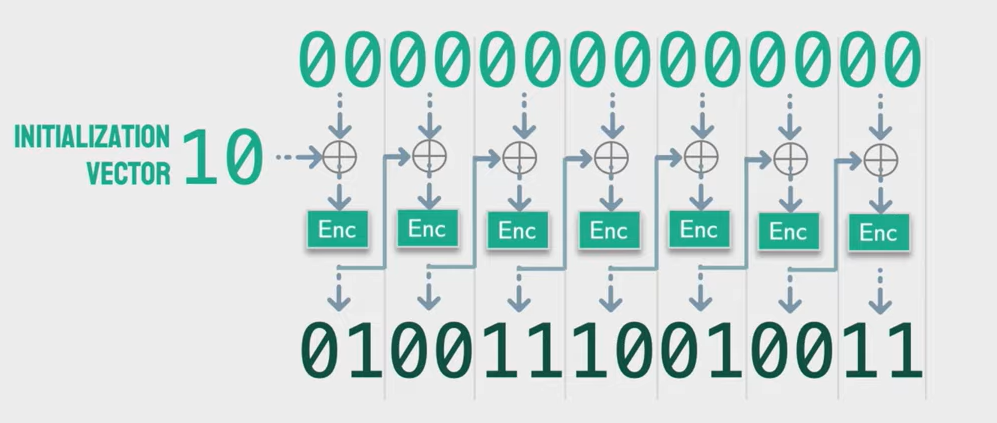
\includegraphics[width=0.6\textwidth]{Photos/Cipher_ Block_Chaining.png}
		\end{SCfigure}
	
		Now another strength of this method is the factor that the same codebook and plaintext can give a wildly different cipher if you just changed the initial seed (or initialisation vector).
		\begin{SCfigure}[0.5][h]
			\caption{This is so nice to look at. Relish the randomness}
			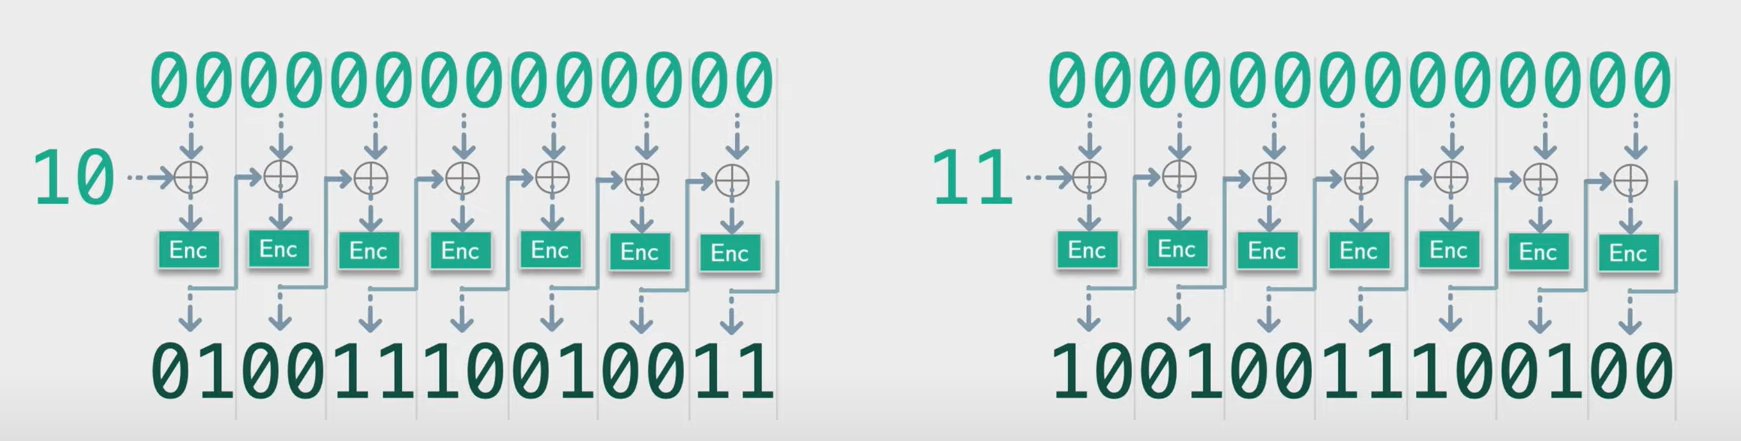
\includegraphics[width=0.6\textwidth]{Photos/CBC_2.png}
		\end{SCfigure}

		\underline{An interesting point}- The I.V. (or initial seed) is not at all a secret. It is in fact given along with the ecrypted message as it is necessary for decryption. Another property - it should not be predictable or used more than once (to ensure resistance from plaintext attacks)

		\subsubsection{How to decrypt CBC}
			\begin{SCfigure}[0.5][h]
				\caption{Decryption exploits the reversibility of \(\oplus\)}
				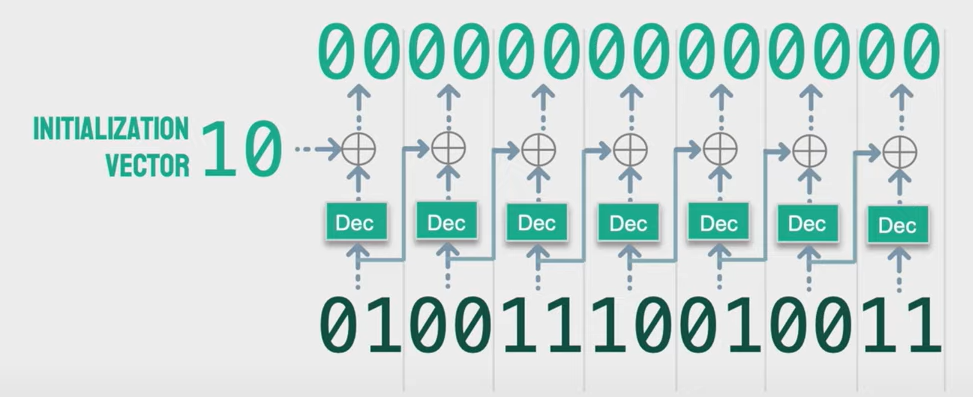
\includegraphics[width=0.6\textwidth]{Photos/CBC_3.png}
			\end{SCfigure}

	\section{Counter Mode (CTR)}
		Another method of Block Ciphering is Counter Mode wherein you are actually encrypting (i.e. using the codebook) on the counter and not the plaintext. The plain text is merely xor-ed with the encryption of the counter. Initial seed decides the starting value of the counter which is incremented.
		\begin{SCfigure}[0.5][h]
			\caption{A very logical and simple encryption process. The counter is on the top and the plaintext is xor-ed in the middle}
			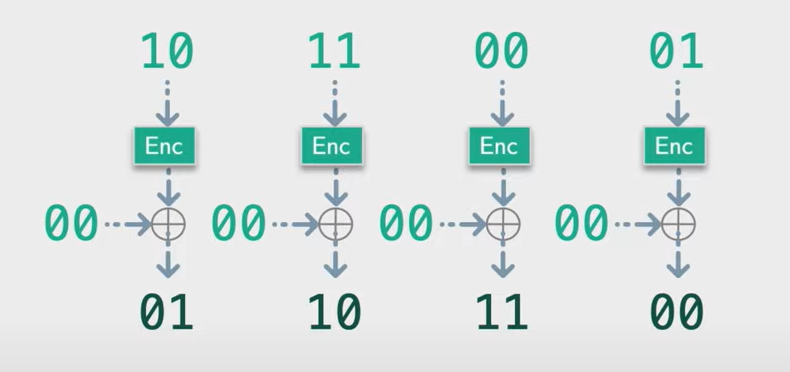
\includegraphics[width=0.6\textwidth]{Photos/CBC_4.png}
		\end{SCfigure}
		
		To put it algebraically, if we called the $k$-bit counter \(C(i)\), and the code book as \(ECB: \{0,1\}^{k} \rightarrow\{0,1\}^k\) and the \(i\)th $k$-bit chunk of plaintext as \(m_i\) then- 
		\begin{mybox}
		\[cipher_i=m_i \oplus ECB(C(i))\]
		\end{mybox}

		\subsection{Decryption}
			\begin{SCfigure}[0.5][h]
				\caption{It is very similar in the sense that we interchange one }
				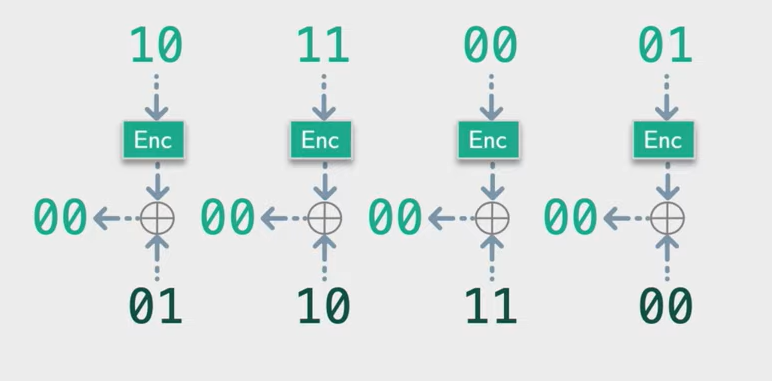
\includegraphics[width=0.6\textwidth]{Photos/CBC_6.png}
			\end{SCfigure}
			In algebraic terms, we can call it- 
			\begin{mybox}
				\[m_i= cipher_i \oplus ECB(C(i))\]
			\end{mybox}

			\begin{center}
			\begin{tabular}{c | c}
				 \hline
				 Advantages over CBC&Disadvantage over CBC\\ 
				 \hline
				 Simpler implementation & Not safe for small block lengths (\(<\)128 bit)\\
				 Resistant to attacks terms as ``padding oracle''& \\
				 \hline  
			\end{tabular}
			\end{center}



    \mychapter{3}{Diffie Hellman and Discrete Logarithms}

\begin{center}
	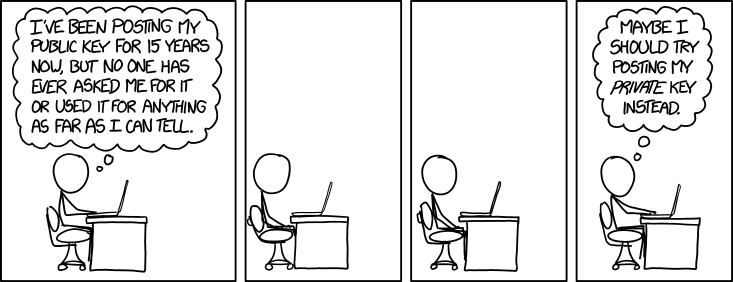
\includegraphics[width=0.75\textwidth]{Photos/Diffie_Hellman.png}
\end{center}

	\mysection{1}{Introduction to Diffie Hellman}
		Finally now we will study a public key cryptosystem in detail. Diffie and Hellman were some of the earliest cryptographers working to create a one-way trapdoor function - easy to compute, difficult to invert unless you have some trapdoor information.
		\begin{SCfigure}[0.5][h]
			\caption{Schematic of a trapdoor function}
			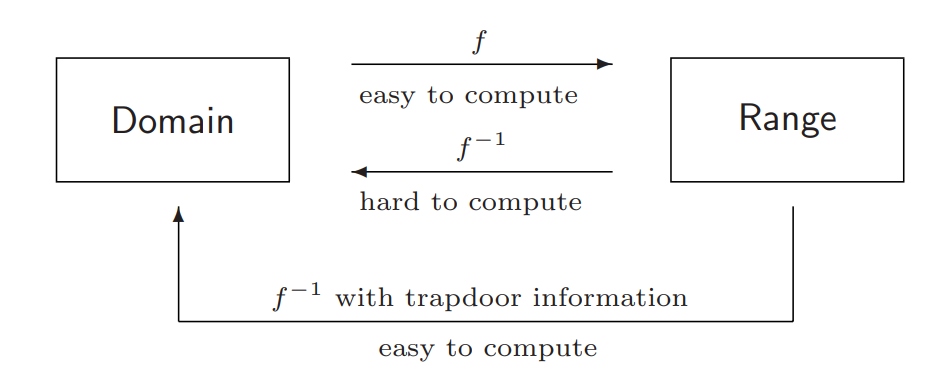
\includegraphics[width=0.6\textwidth]{Photos/DH_1.png}
		\end{SCfigure} 

		These functions are of a particular importance. As was explained in \textcolor{teal}{\hyperref[sec:asym]{Asymmetric Ciphers}} section, we make sure of \(k_{public}, \; e_k()\) for encryption which is made public knowledge whereas \(k_{private},\; d_k()\) are kept private as they are used for decryption. Since \(k_{public}\) is constructed from \(k_{private}\), it is important that the function that decides their relation is unidirectional else finding \(k_{private}\) will be possible for \(Eve\) from just the information that is publically available.

		\begin{mybox}
			\textbf{Why exactly is the use of public key cryptography even?}
			\tcblower
			Banks in the internet age would require to hand deliver keys to their clients which would massively slow down communications and created massive weaknesses in the line of communication. Hence finding a solution to this problem was important.
		\end{mybox}

		\quad But another thing to keep in mind is that if \(Bob\) is receiving the message from \(Alice\), he should be able to decrypt it since he has that extra information. \par

		Although ultimately Diffie and Hellman failed to create a public key cryptosystem (PKC), they did manage to create a system that can securely transfer certain data by utilising the Discrete Logarithm problem.

	\mysection{2}{Discrete Logarithm}
		Refer to \textcolor{teal}{\hyperref[sec:prime]{Prime numbers and Finite Fields}} for the background information in this section. According to the \textcolor{teal}{\hyperref[subsec:primitive]{Primitive Roots Theorem}}, in every \(\mathbb{F}_p\), there exists a \(g\) such that \(1, g^1, g^2, \ldots , g^{p-1}\) contains all the elements present in \(\mathbb{F}_p*\) and \(g^{p-1}\equiv 1 \bmod(p)\) (\textcolor{teal}{\hyperref[sec:fermat]{Fermat's Little Theorem}}).\par
		\emph{Discrete Logarithm Problem} (DLP) is the problem of finding \(x\) such that- \[g^x \equiv h \bmod(p)\] for some arbitrary \(h\) and \(x\) is called the \emph{discrete logarithm of h to the base g} \(= \log_g{h}\).\par
		\begin{mybox}
			\[x= \log_g{h} \bmod(p)= \text{Discrete logarithm(} h \text{)} \quad \text{for } x, h \in \mathbb{F}_p^*\]
		\end{mybox}
		\begin{tcolorbox}
			\textbf{\underline{Note-}} We use the term ``index'' to sometimes refer to the discrete logarithm i.e. \(x=\text{ind}_g{(h)}\). This is to ensure that the usual log and discrete log are not confused for each other.
		\end{tcolorbox}
		\(x' = x + (p-1) k \) would also satisfy our condition thus giving up \(\infty\)ly many solutions $x$. Hence \(x\) is only defined modulo (p-1). Hence we say that \[\text{ind}_g : \mathbb{F}_p* \rightarrow (\mathbb{Z}/(p-1)\mathbb{Z})\]
		\subsection{Why is it called logarithm?}
		Well you can easily see that \[\text{ind}_g (ab)=\text{ind}_g (a)+\text{ind}_g (b)\] and that gives us enough of a reason to call it so.

		\begin{tcolorbox}[breakable, title=Illustration,colback=brown!5!white,colframe=brown!75!black,colbacktitle=yellow!50!red,coltitle=red!25!black,fonttitle=\bfseries,subtitle style={boxrule=0.4pt,colback=yellow!50!red!25!white} ]
			If our prime number \(p = 56509\), and we know with surety that \(g = 2\) is a primitive root modulo \(p\), we can be sure that \(2\) is a ``generator'' of (\(\mathbb{Z} / p \mathbb{Z}*\)) hence the discrete logarithm of every number \(< p\) to the base \(2\) exists.

			In that case, if we have to calculate \(\text{ind}_2{38679}\), we will have to cycle through \textbf{every} one of \(1,2,2^2, 2^3, \cdots 2^{56508} \bmod(56509)\), until we get a value that matches \(38679\). This is exactly why the discrete logarithm problem is a formidable one.
			
			\tcbsubtitle{How did we know that 2 is a primitive root modulo 56509?}
				If we wanted to check if a number \(a\) is a primitive root modulo \(p\), the first approach that comes to mind might be to first evaluate all powers of \(a\) modulo \(p\) from 0 to \(p-2\) and see if all numbers from 1 to \(p-1\) appear exactly once. But this is too resource consuming so we use a better approach. 
				Since we know that if \(a\) is really a primitive root, then all the powers of \(a\) modulo \(p\) would be a bijective function with the set \({1, 2, 3, \cdots, p-1}\), we can be sure that 1 would appear once in the powers other than the \(p-1\)th power. (If 1 does not appear even once in between 0 and \(p-1\), we can be sure that all the values will \textbf{have} to be unique hence making \(a\) a primitive root).
				So we have \[a^{p-1} \equiv 1 \bmod(p)\] So we just have to calculate the prime factors (\(q_1, q_2, ...\)) of \(p-1\) and if 
				\[a^{\frac{p-1}{q_i}}\not \equiv 1 \bmod(p) \quad \forall i \text{ such that } q_i \text{ divides } p-1 \Rightarrow a \text{ is a primitive root modulo } p\] 

			\tcbsubtitle{Is it necessary for \(g\) to always be a primitive root modulo p?}
				No. As long as 2 things are ensured, we can always write \(\text{ind}_g{h}\)-
				\begin{enumerate}
					\item The discrete logarithm exists. \\e.g. In \hyperref[example:six]{this example}, \(\text{ind}_62\) is just not defined.
					\item The value is unique (in ring \(\mathbb{Z}/ p \mathbb{Z}\)) \\ e.g. In the \hyperref[example:six]{same example}, we can see that \(\text{ind}_66\) will have multiple values (1, 3, 5).
				\end{enumerate}
		\end{tcolorbox}

		The strongest point of our encryption using Discrete Logarithm is that there is a lot of variation and a seeming randomness in the values of the discrete logarithms in our data.
		\begin{SCfigure}[0.5][h]
			\caption{Table of values of \(h\) for \(g = 627\) and \(h= 941\)}
			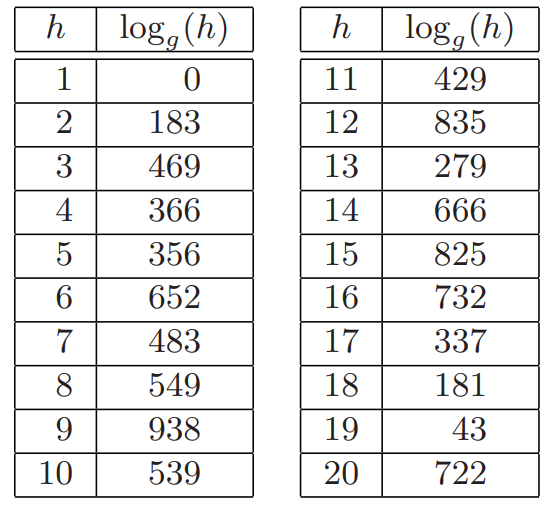
\includegraphics[width=0.4\textwidth]{Photos/Discrete_log_1.png}
		\end{SCfigure}

	\mysection{3}{Using Discrete Logarithm for Key Exchange}
		Let us say that \emph{Bob} and \emph{ALice} want to begin communication across an insecure channel. If they can agree upon a key, the communication can begin smoothly using any of the block or stream cipher ways we have already discussed. But how do you send the key, very well knowing that any and all information across the channel can easily get intercepted? \par
		In that case, \emph{Bob} and \emph{Alice} publicly agree upon \(g\) and \(p\). \emph{Alice} and \emph{Bob} then privately construct some \(a\) and \(b\) respectively without letting it be known to the outside world. \par
		\emph{Bob} then sends \emph{Alice} \(A = g^a \bmod(p)\) and \emph{Alice} sends back \(B = g^b \bmod(p)\). Due to the nature of the insecure channel, \emph{Eve} is able to safely intercept both \(A\) and \(B\). \par
		Finally \emph{Alice} calculates \(B^a \bmod(p)\) and \emph{Bob} calculates \(A^b \bmod(p)\). It is obvious that even in \(\mathbb{F}_p\), \(A^b = g^{ab} = B^a \bmod(p)\) hence that becomes the key the both parties use for secure communication henceforth.
		\emph{Eve}, despite knowing \(A, B, g\) and \(p\), is still unable to calculate \(g^{ab} \bmod(p)\) trivially because of her not knowing the values \(a\) and \(b\).

		\begin{center}
			\begin{tabular}{ c | c | c}
				 \hline
				 Information \emph{Bob} has & Information \emph{Alice} has & Information \emph{Eve} has\\ 
				 \hline
				 \hline
				 \multicolumn{3}{c}{\textbf{Before exchange}}\\
				 \hline
				 \(b,\; g,\; p,\; B\; (=g^b \bmod(p))\) & \(a,\; g,\; p,\; A\; (=g^a \bmod(p))\) & \(g,\; p\) \\
				 \hline
				 \multicolumn{3}{c}{\textbf{After exchange}}\\
				 \hline  
				 \(b,\; g,\; p,\; B,\; A\) & \(a,\; g,\; p,\; A,\; B\) & \(g,\; p,\; A,\; B\) \\
				 \multicolumn{2}{c}{Key (=\(A^b = B^a =g^{ab}\))} & No information about the key
			\end{tabular}
			\end{center}

		\begin{tcolorbox}[breakable, title=Does this mean that finding the key is a Discrete Logarithm Problem (DLP)?,colback=red!5!white,colframe=red!75!black]
			No. \\
			If the only way for \emph{Eve} to find the key was to find out \(a\) from \(A\) and \(g, p\) (or similarly \(b\) from \(B\) and \(g , p\)), then admittedly, this problem would have been a classic DLP problem.\par However, \emph{Eve} actually has both \(A\) and \(B\) and thus actually has to find \(g^{ab}\) using \(g^a\) and \(g^b\) which is definitely a simpler problem. This problem is termed as the \textbf{Diffle Hellman Problem} (DHP) and is not harder than the DLP.
			\tcblower
			We called DHP to be ``not more difficult than'' DLP instead of saying DHP is easier than DLP. The reason for it is that although we know if DLP was computable, DHP would be trivially solvable, the converse hasn't been proven.
		\end{tcolorbox}

		\begin{tcolorbox}
			For the modern standards of computing power, \(p\) needs to be \(\approx 1000\) bits for brute-force to not be a feasible option in \emph{Eve}`s hands. Also, \(g \approx p/2\) ensures most computational difficulty in the inversion of Discrete Logarithm.
		\end{tcolorbox}

		\centering{\Huge{\textcolor{orange}{But wait!}}} \par
		\raggedright \noindent Doesn't this mean we can effectively create a \emph{\hyperref[box:onetimepad]{One Time Pad}} (OTP) and hence an indecipherable means of communication is feasible using DHP? \\
		Yes, but also no.\footnote{At this point, the reader should just get used to seeing every question mark and brace themselves for a \hyperref[box:whyno]{heartless ``No.''}}\\
		Although it is very much possible to have a system wherein, 
		\begin{itemize}
			\item If \emph{Alice} and \emph{Bob} agree on only sharing 160-bit messages, they publicly choose a large enough (\(\approx 160\) bit)\(p, g\).
			\item Then both of them use \hyperref[subsec:prng]{PRNGs} privately to construct \(a, b\) of a suitable size so as to ensure that the final \(g^{ab}\) has a length larger than 160-bits.
			\item If the key has more than 160 bits, chop off the last few bits until you get a key \(k'\) of exactly 160 bit size.
			\item Use $\oplus$ (\text{xor}) on \(k'\) and \(m\) and then if \emph{Alice} sends this encrypted message to \emph{Bob}, \emph{Bob} can just calculate \(k' \oplus c \equiv m\) to get the original message.
			\item \emph{Alice} and \emph{Bob} change keys thus \(a\) and \(b\) for every message sent across the channel thus ensuring that they create a feasible One-Time Pad encrypted network.
		\end{itemize}

		\begin{mybox}\label{box:whyno}
			Although the above method is really great, it is not a secure system in today's times. The flaws this suffers from can best be explained at the \hyperref[sec:whydiffiesucks]{end of this chapter}.
		\end{mybox}

		\subsection{The anti-climactic conclusion of Diffie-Hellman}
			As you will come to see in the further sections, certain cases of Diffie Hellman are feasible to solve really quick and others can be solved with more efficient algorithms. There also exist some other flaws which prevent Diffie Hellman, despite all its glory, from becoming the cryptosystem standard it deserved to be. Rest in Peace :(

	\mysection{4}{ElGamal Public Key Cryptography}
		Fear not, for now we have a different approach to use the Discrete Logarithm Problem without having to sacrifice either speed or security (we don't want it to be any simpler to solve than the \textbf{DHP}).\\
		The steps for setting up an ElGamal Cryptosystem is as follows-
		\begin{enumerate}
			\item \emph{Alice} and \emph{Bob} agree on a \(g\) and a large enough \(p\).
			\item \emph{Alice} randomly\footnote{Of course, pseudo-randomly using a suitable \hyperref[subsec:prng]{PRNG} or such} chooses an \(a\) and publicly displays \(A \equiv g^a \bmod(p)\).
			\item \emph{Bob} then randomly\footnote{Again the same misnomer as above.} creates a \emph{ephemeral key} \(k\) (which will be used for this message only). 
			\item \emph{Bob} can only encrypt a message \(2< m < p\). He does so by calculating the 2 following values \(c_1 \equiv g^k \bmod(p)\) and \(c_2 \equiv m \cdot  A^k \bmod(p)\).
			\item He then sends \(c_1\) and \(c_2\) to \emph{Alice} who then can calculate \(m \equiv (c_1^a)^{-1} \cdot c_2 \bmod(p)\).
		\end{enumerate}

		\begin{mdframed}
			\centering \textbf{Proof of the above-}
			\[c_1^k \equiv g^{ak} \Rightarrow (c_1^k)^{-1} \equiv (g^{ak})^{-1} \bmod(p)\]
			\centering
				AND
			\[c_2 \equiv m \cdot (g^a)^k \equiv m \cdot g^{ak} \bmod(p)\]
			\raggedright Hence
			\[(c_1^a)^{-1} \cdot c_2 \bmod(p) \equiv (g^{ak})^{-1} \cdot m \cdot (g^{ak}) \equiv m \bmod(p)\]
		\end{mdframed}

		\begin{tcolorbox}[breakable, colback=blue!5!white,colframe=blue!75!black]
			Since \(c_1\) and \(c_2\) are of the same range of bits as \(m\), in order to send one bit of data, we send 2 bits of encrypted bits hence it is called a \emph{2-to-1 message expansion}.
		\end{tcolorbox}

		ElGamal Cryptography is as secure as the Diffie Hellman problem - i.e. in order to decrypt a ElGamal encrypted code, you need to solve the Diffie Hellman problem.\footnote{An intuitive proof would be- assume you have a machine that can decrypt any ElGamal encrypted data if you supplied it the necessary \(c_1\) and \(c_2\). In that case, providing \(c_1 = B\) and \(c_2 = 1\) just gives us \((c_1^a)^{-1}\cdot c_2 \equiv (g^{ab})^{-1} \bmod(p)\) hence giving us the Diffie Hellman key essentially.}

	\begin{mdframed}
	\mysection{5}{Mathematical Pre-requisite: Group Theory}
		\subsection{General properties of a Group}
			A group consists of a set $\mathbf{G}$ and a rule, which we denote by \(\star\), for combining two elements $a,b \in \mathbf{G}$ to obtain an element \(a\star b \in \mathbf{G}\). The composition operation \(\star\) is required to have the following three properties:
			\begin{itemize}
				\item \textbf{Identity law-} There exists an \(e \in \mathbf{G}\) such that, for every \(a \in \mathbf{G}\), \[a\star e = e \star a= a\]
				\item \textbf{Inverse law-} There exists a unique \(a^{-1} \in \mathbf{G}\) for every \(a \in \mathbf{G}\) such that, \[a \star a^{-1}= a^{-1} \star a = e\]
				\item \textbf{Associative law-} For every \(a, b, c \in \mathbf{G}\), \[a\star(b\star c )=(a\star b)\star c\]
				\item \textbf{Commutative law-} (optional- if group follows this as well, it is called a \emph{Commutative} or \emph{Abelian Group}) For every \(a, b \in \mathbf{G}\), \[a\star b = b \star a\] 
			\end{itemize}
			
			\begin{tcolorbox}
				Order of a group
				\tcblower
				\(|\mathbf{G}|\) or \(\# \mathbf{G}\) is the \emph{order of group \(\mathbf{G}\)} and it is the number of elements present in \(\mathbf{G}\). \(\mathbf{G}\) is called a \emph{finite group} if \(\# \mathbf{G} \in \text{finite} \mathbb{N}\). 
			\end{tcolorbox}

			\textbf{Examples-}
			\begin{enumerate}
				\item \(\mathbb{F}_p^*\) is a finite group, with order \((p-1)\) with composition operation \(\star = \times\) (multiplication). \(e=1\) and inverses do exist.
				\item \(\mathbb{Z}\) has \(\star = +\) (addition) and is an infinite group. \(e = 0\) and inverse of \(a \Rightarrow -a\)
				\item \(\mathbb{Z}\) with \(\star = \times\) is not a group since inverses do not exist inside the group for every element.
				\item A non commutative group can be \(\mathbf{G} = \begin{cases}\big(\begin{smallmatrix}
				  a & b\\ 
				  c & d
				\end{smallmatrix}\big)\end{cases} ; (ad-bc \not = 0)\). It has \(e = \big(\begin{smallmatrix}
				  1 & 0\\ 
				  0 & 1
				\end{smallmatrix}\big)\) and since \(\text{det}(A) \not = 0\) where \(A \) is a matrix \(\in \mathbf{G}\), an inverse also exists.
			\end{enumerate}

			If \(g\) is an element of \(\mathbf{G}\), \(g^x\) denotes \[\underbrace{g\star g\star g\star \cdots \star g}_{\text{x times}}\]
			\begin{itemize}
				\item[\(\#\)] \(g^0 = e\)
				\item[\(\#\)] If \(x<0\), we define \(g^x\) as \((g^{-1})^{|x|}\)
				\item[\(\#\)] Even though it may seem non-intuitive, \(g^x\) for \(\begin{cases}\mathbf{G}= \mathbb{Z}\\ \star=+ \end{cases}\) is actually \(g+ g+ g+ \cdots=x\cdot g\)
			\end{itemize}

			\begin{mybox}
				If \(a\in \mathbf{G}\), and if \(d\) is the smallest positive integer such that, \[a^d=e\] then \(d\) is called \textbf{order of a}. If no such \(d\) exists, \(a\) is said to have \textbf{infinite order}.
			\end{mybox}

			\subsection{Generalisation of Fermat's ``Little'' Theorem}
				
				If \(\mathbf{G}\) is a finite group, then every element \(\in \mathbf{G}\) will have finite order. \\ Furthermore, if \(a \in\mathbf{G}\) and has order \(d\), and\footnote{Trivial proof: Since \(d\) is the smallest positive integer which ensures \(a^d=e\), if we wrote \(k=q\cdot d + r\), where \(0<r<d\), then obviously \(a^k \not = e\)} \[a^k = e\Rightarrow d\;|\;k\]
			
			\begin{tcolorbox}[title=Lagrange's Theorem,colback=green!5!white,colframe=green!75!black]\label{theo:LagrangeTheo}
				Let \(\mathbf{G}\) be a finite group and let \(a \in \mathbf{G}\). Then the order of $a$ divides the order \(\mathbf{G}\).\footnote{Proof: If \(a\in\mathbf{G}=\{g_1, g_2, g_3, \cdots, g_n\}\), we can construct a new group \(\mathbf{S_a}=\{a\star g_1, a\star g_2, \cdots, a\star g_n\}\). Now using the definition of group (If \(a, b\in \mathbf{G}\), \(a\star b \in \mathbf{G}\) as well) we can be sure that every element of \(\mathbf{S_a}\) is an element of \(\mathbf{G}\) as well since \(a \in \mathbf{G}\). Keeping that in mind, \[a\star g_1 \times a\star g_2 \times \cdots \times a\star g_n = g_1 \times g_2 \times \cdots \times g_n\] Now we assume our group is Commutative (more general proof is slightly more rigorous) hence we can say that \[a^n = e\]}
				\tcblower
				\normalsize In other words, if \(|\mathbf{G}|=n\), then \[a^n=e \text{ AND } d\;|\;n\]
			\end{tcolorbox}
	\end{mdframed}

	\mysection{5}{How difficult is the DLP?}
		Up until now, we have claimed that the DLP is a very difficult problem. Now it is time to quantify the difficulty using big-\(\mathcal{O}\) notation.

		\subsection{Big- \(\mathcal{O}\) notation}
			\begin{tcolorbox}
				\textbf{Formal definition.} If $f(x)$ and $g(x)$ are 2 positive functions, $f(x)$ is called ``big-\(\mathcal{O}\) of $g(x)$'' iff there exists a positive $C,\; k$ such that \[|f(x)|\leq C\cdot |g(x)| \forall x>k\]
				\tcblower
				In other words, $f(x)= \mathcal{O}(g(x))$ iff \[\lim_{x\to\infty} \bigg|\frac{f(x)}{g(x)}\bigg|\text{ exists and is finite}\] 
			\end{tcolorbox}

			\textbf{\underline{Some examples}}-
			\begin{itemize}
				\item \(x^2 + 3x + 2981= \mathcal{O}(x^2)\)
				\item \((\log x)^{375} = \mathcal{O}(x^{0.001})\)
				\item \(x^2 \cdot 2^x= \mathcal{O}(e^x)\)
			\end{itemize}

			Although this is the mathematically pure definition, we will use a slightly different definition somewhat loosely while we talk of difficulty in the proceeding sections -

			\begin{mybox}
				\textbf{``Definition''.} If we made a proper list of ``complexities'' ($0, 1, \log n, n, n^2, n^3, \ldots 2^n, \ldots, n!, n^n\ldots$), and if \(f(x) = \mathcal{O}(g(x))\),  \(g(x)\) has to be the ``least complex'' function which satisfies the previous formal definition.
				\tcblower
				In other words, $f(x)= \mathcal{O}(g(x))$ iff \[\lim_{x\to\infty} \bigg|\frac{f(x)}{g(x)}\bigg|\text{ exists and is \textcolor{red}{non-zero} finite}\]
			\end{mybox}

			If an algorithm has an input of \(k\)-bits, then if output has order-
			\begin{itemize}
				\item[--] \(\mathcal{O}(k^a)\) where \(a \in \text{positive constant}\): Polynomial order \(\to\) ``Easy'' Problems
				\item[--] \(\mathcal{O}(e^{ax})\) where \(a \in \text{positive constant}\): Exponential order \(\to\) ``Hard'' Problems 
				\item[$\#$] There also exists a ``Sub-exponential order'' can be best described as ``grows faster than any polynomial function but slower than \textbf{any} exponential function of the form \(b^x \quad\forall b>1\).''
			\end{itemize}

		\subsection{Computing \(\mathcal{O}\) for DLP}
			\[g^x=h \text{ where }g\in\mathbf{G}=\mathbb{F}_{p}^{\ast} \text{ and } \star= \times \Rrightarrow \text{Finding \(x\), given \(g, p, h\)} \quad \cdots (\text{DLP})\]
			If \(p \in (2^k, 2^{k+1})\), then obviously \(p, g, h\) all will take individually \(k\)-bits at most. Thus we can say that input/data we are dealing with is \(\mathcal{O}(k)\).\par
			Using trial-and-error method, we will, in the worst case scenario, be evaulating all of the \((p-1)\) numbers from \(1\) to \(p-1\) hence order\( =\mathcal{O}(p)= \mathcal{O}(2^k)\) hence exponential \(\rightarrow\) \textcolor{red}{difficult}.\par
			But that is not the only approach we have in hand.
			\begin{itemize}
				\item[\(\ast\)] For some primes, where \(p-1\) can be factored into a product of small primes, we can use the \hyperref[sec:pohlig]{\emph{Pohlig-Hellman}} algorithm which makes the DLP for them quite \textcolor{red}{easy}.
				\item[\(\ast\)] \hyperref[sec:colli]{\emph{Collision algorithm}} works for all primes and takes \(\mathcal{O}(\sqrt{p} \log p)\) steps (still exponential but \textcolor{red}{easier than} \(\mathcal{O}(p)\))
				\item[\(\ast\)] Using index calculus, we can bring it down to \(\mathcal{O}(e^{c\sqrt{(\log p)( \log\log p )}})\) which is \textcolor{red}{sub-exponential}.
			\end{itemize}

		\subsection{How there is no inherent difficulty in DLP}
			The last few sections about DLP in \(\mathbb{F}_p^*\) might give you an impression that all DLPs of the form \(g^x = h \quad g, h\in \mathbf{G}\) are inherently difficult. \par
			In constrast, if \(\mathbf{G}=\mathbb{F}_p\) and \(\star = +\), our DLP can also be written as \[x \cdot g = h \bmod(p)\]
			Now using \hyperref[theo:extendedEuclid]{Extended Euclidean Theorem}, we know that finding \(g^{-1}\) in the above setup will take \(\mathcal{O}(\log p) = \mathcal{O}(\log 2^k)\) steps thus is solvable in \textcolor{red}{linear time}.

			With index calculus, DLP for \(\mathbf{G}=\mathbb{F}_p^*\) and \(\star=\times \) is solvable in \textcolor{red}{sub-exponential time}.

			If we instead had \emph{Elliptic curves}, our best algorithm for DLP takes \textcolor{red}{exponential time}.

	\mysection{6}{Collision Algorithm}\label{sec:colli}
		Collision Algorithms work by creating 2 lists, of approximately the same size for maximum efficiency and then comparing the 2 lists. This is considerably faster than just trial-and-error method we evaluated until now.

		\begin{tcolorbox}[breakable, title=Shank's ``Babystep- Giantstep'' Theorem,colback=blue!5!white,colframe=blue!75!black]
		 	Let \(g \in \mathbf{G}\) be an element of order \(N >2\). Then we can employ the following algorithm to get order of \(\mathcal{O}(\sqrt{N} \cdot \log N)\)\footnote{Proof: Making each list takes $n$ multiplications each (\hyperref[subsec:fastexpo]{fast powering algorithm}) and sorting and searching through the list takes another \(\mathcal{O}(\log n)\) steps- bringing the total time to \(\mathcal{O}(n \log n)= \mathcal{O}(\sqrt{N} \log N)\)}-
		 	\begin{enumerate}
		 		\item Let \(n = 1 + \lfloor\sqrt{N}\rfloor\) i.e. \(n> \sqrt{N}\).
		 		\item Then construct 2 lists- \[\text{List$_1$}= e, g, g^2, g^3, \ldots g^n\] \[\text{List$_2$}= h, h\cdot g^{-n}, h\cdot g^{-2n},
		 		\ldots , h\cdot g^{-n^2}\] 
		 		\item Now try to find the common entry in both lists. There should exist just one pair such that \[g^i = h \cdot g^{-j \times n}\]
		 		\item Then \(x = i + n \times j\) is the solution to \(g^x = h\).
		 	\end{enumerate}
		 \end{tcolorbox}
		 
		 \begin{mybox}
		 	\textbf{Intuitive explanation for how this works:} \\
		 	First of all, the size of \(\mathbf{G}\) does not matter since, if \(h\) is a valid solution of \(g^x = h\), \(x\) will have exactly one solution per \(N\) per values of $x$ we cycle through. We will only concentrate on the first \(N\) values i.e. the first \(x\) that satisfies our condition.\vspace{0.5cm}

		 	Moreover, we can write \(x= p \cdot n + q\) and since \(x\leq N \text{ AND } n>\sqrt{N}\text{, }p<\sqrt{N}\) and by remainder theorem, \(q<n\Rightarrow q<\sqrt{N}\). Hence if there was a way to make 2 lists such that one decides $p$ and the other sets $q$, our inversion algorithm would be successful.\vspace{0.5cm} 

		 	Hence we find \(u = (g^{-1})^n\) (which due to the \hyperref[theo:extendedEuclid]{extended Euclidean theorem}, is easy to compute) and then just find \(h, h\cdot u, h\cdot u^{2}, \ldots , h \cdot u^{n} \Rrightarrow \text{List}_2 \text{ a.k.a. $p$ setter}\). \(\text{List}_1\) is just \(e, g, g^2, \ldots, g^n\) which is the $q$ setter.\vspace{0.5cm}

		 	Finally when they correspond, \(h\cdot u^{p}=h\cdot (g^{-1})^{p\cdot n}= g^q \Rightarrow h = g^{p \cdot n + q}= g^x\)
		 \end{mybox} 
		 \begin{center}
		 	\Huge \textcolor{orange}{Jargon Overload}\\
		 	\normalsize That was a lot of jargon. Let's take a look at an example for better understanding.
		 \end{center}

		 \begin{tcolorbox}[breakable, title=Illustration,colback=brown!5!white,colframe=brown!75!black,colbacktitle=yellow!50!red,coltitle=red!25!black,fonttitle=\bfseries,subtitle style={boxrule=0.4pt,colback=yellow!50!red!25!white} ]
		 	In DLP, take \(\mathbf{G}=\mathbb{F}_p^*\) and \(\star=\times\) with \(p = 17389\), \(g= 9704\), and \(h=13896\). Find a suitable \(x\).
		 	\tcblower
		 	Order of \(g=9704\) in \(\mathbb{F}_{17389}^*\) is $1242$.\footnote{How did we get this order? \\The standard algorithm is to try and break \(17388\) into its prime factors and then try them one by one till the smallest factor \(k\) yields $g^k = e$. (Reason- Size of the group is 17388 hence using the \hyperref[theo:LagrangeTheo]{Langrange's Theorem}, we can be sure that the order is a factor of order of the group)}

		 	Using that, \[n = \lfloor\sqrt{N}\rfloor+1= 36\]
		 	Next, \[u=(9704^{-1})^{36}\]
		 	We find \(9704^{-1}\) using recursion with \hyperref[theo:extendedEuclid]{Extended Eucleadian Theorem} in linear time. After that, we just use \hyperref[subsec:fastexpo]{Fast Powering Algorithm} to find \(u\).\\
		 	That yields us \[u = 2494\]
		 	Now we constuct the two lists- 
		 	
		 	\begin{center}
		 		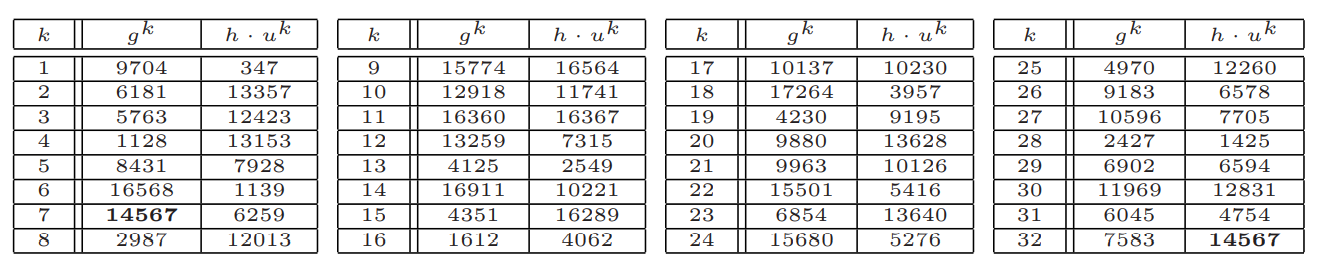
\includegraphics[width=0.8\textwidth]{Photos/DH_2.png}
		 	\end{center}

		 	As you can clearly see, \[9704^7=14567=13896 \cdot 2494^{32}= 13896 \cdot (9704^{-36})^{32}\Rightarrow13896= 9704^{1159}\Rightarrow x=1159\]
		 \end{tcolorbox}

	\mysection{7}{Congruences moduli composite numbers}
		Up until now, we have only dealt with congruences of the form \(\bmod(p); \: p \in \text{primes}\). But, what if we have to do computations in \(\bmod(m);\: m \not\in \text{primes}\)? Well that is where we get a helpful hand from the Chinese Remainder Theorem.
		
		\begin{mdframed}
			\subsection{Chinese Remainder Theorem}\label{subsec:chinese}
				Suppose you are given- \[x \equiv a \bmod(p) \text{ AND } x \equiv b \bmod(q) \text{; where $p$, $q\in $ primes}\]
				We can use this information to find the value of \textcolor{orange}{\(x \bmod(p\cdot q)\)}. 
				
				\textbf{Algorithm:}
				\begin{enumerate}
					\item Since \(x\equiv a \bmod(p)\), we can write \(x = a + p \cdot y\).
					\item Input that in the second congruence to get \(p \cdot y \equiv b -a \bmod(q)\). Now since \(\gcd(p,q)=1\) (prime numbers, duh), we know that \(p^{-1}\) exists.
					\item Hence finally we get \(y \equiv p^{-1}(b-a)\bmod(q)\)
					\item Assuming \(y<q\), we input the RHS into \(x= a + p \cdot y\) and viola! We just got a value of \(x\) in modulo \(p\cdot q\) (since, if \(c_1\) and \(c_2\) are solutions of \(x\) in this situation, \(c_1 = k\cdot (p\cdot q) + c_2\))
				\end{enumerate}
				\begin{tcolorbox}[breakable, title=Illustration,colback=brown!5!white,colframe=brown!75!black,colbacktitle=yellow!50!red,coltitle=red!25!black,fonttitle=\bfseries,subtitle style={boxrule=0.4pt,colback=yellow!50!red!25!white} ]
					\[x\equiv 1 \bmod(5) \text{ AND } x \equiv 9 \bmod(11)\]
					Thus \[x = 1 + 5 y\Rightarrow 5 y \equiv 8 \bmod(11)\]
					Now \(5^{-1}=9\). Using that, \[y \equiv 72 \bmod(11)\equiv 6 \bmod(11)\]
					Finally \(y =6 \Rightarrow x = 31\) is a particular solution. The final answer is-\[x\equiv 31 \bmod(55) \Leftrightarrow x = 31 + 55k \]
				\end{tcolorbox}

				Extending it to multiple numbers is just iteratively i.e. if \(\gcd(m_1, m_2, m_3, \ldots, m_i)=1\), \(x\equiv a_1\bmod(m_1)\), \(x\equiv a_2\bmod(m_2)\), \(x\equiv a_3\bmod(m_3)\), ... , \(x\equiv a_i\bmod(m_i)\). Now just try to find \(x \bmod(m_1\cdot m_2)\) and then continue accordingly since \(\gcd(m_1\cdot m_2, m_3)=1\).
		\end{mdframed}

		And thus we can just decompose any \(m\) into a product of primes and then apply Chinese Remainder Theorem. 

		\subsection{Application of CRT}			
			A good use\(\Rightarrow\) Finding square roots in modulo $m$. It is actually easy to calculate square roots in modulo prime, and more so in primes of form \(4l + 3\). \\ If \(x^2 \equiv a \bmod(p)\), then we can write that \(x\equiv a^\frac{p+1}{4} \bmod(p)\) \par
			How? Well, if we assumed \(g\) is the primitive root modulo \(p\), we can write \(x \equiv b \equiv g^k\) as a solution. Then, \[x^2 \equiv a^\frac{p+1}{2} \equiv a^\frac{p-1}{2} \cdot a \equiv g^{k \cdot (p-1)}\cdot a \equiv 1 \cdot a \bmod(p) \]
			Using this, if we had to solve for \(x^2 \equiv a \bmod(m)\) where \(m = p_1 \cdot p_2\), if they are of the form \(4\alpha +3\), we can easily write, \[x\text{ can be found by solving the congruences of $y$ and $z$} \text{ where } y^2 \equiv a \bmod(p_1)\text{ and } z^2 \equiv a \bmod(p_2)\] We can solve according to the previously discussed method. \par
			\textbf{Note:} \(x^2 \equiv a \bmod(p)\) will have 2 solutions but the above one will have 4 solutions since we can solve 4 different final congruences based on + - changes.
		\begin{mybox}
			Factorisation of \(m\) isn't really easy as \(m\) increases in size. In that case, directly evaluating whether or not the roots exist or not becomes really a tedious task. We can use that to construct a trapdoor function-  \href{https://bit.ly/3IFyTW7}{``Goldwasser–Micali'' Cryptosystems}\footnote{\cite{IIScGold}} depend on this function with the trapdoor information being the factors of \(m\).
		\end{mybox}

	\mysection{8}{Pohlig-Hellman Algorithm} \label{sec:pohlig}
		Pohlig-Hellman first starts off by analysing the fact that when we are talking about solutions of \(g^x \equiv h \bmod(p)\), \(x \in \mathbb{Z}/(p-1)\mathbb{Z}\) since \(x = p-1\) will just give the same value as \(x = 0\). So we try to exploit the fact that \(p-1\), an obviously composite number has prime roots and hodge podge a solution using \hyperref[subsec:chinese]{Chinese Remainder Theorem}.\par
		Let us first start off with an example instead of the actual theory. 

		\begin{tcolorbox}[breakable, title=Illustration,colback=brown!5!white,colframe=brown!75!black,colbacktitle=yellow!50!red,coltitle=red!25!black,fonttitle=\bfseries,subtitle style={boxrule=0.4pt,colback=yellow!50!red!25!white} ]
			
			Given that \(2\) is a generator of 211 (a.k.a. primitive root modulo 211), find \(x\) such that\footnote{Example was taken from \href{https://bit.ly/3O8XIKX}{this video}.} \[2^x \equiv 41 \bmod(211)\]
			\textbf{Proof:}\\
			Since we know that $2$ is a generator, we can be sure that a solution exists. Now, let us suspend belief for a few fleeting seconds and just find the roots of \(\phi(211)= 210\). The factorisation yields \(210 = 2\cdot 3\cdot 5\cdot 7\).\\
			Again, as a leap of faith just find \(a^\frac{\phi(p)}{7} \bmod(p)\) (for sake of simplicity, refer to \(211\) as $p$ and \(a \equiv 2^x \equiv 41\))
			\[a^\frac{\phi(p)}{7}\equiv (2^x)^\frac{\phi(p)}{7} \bmod(p) \]
			\[\text{Using remainder theorem, write } x=7q +r \Rightarrow 2^{q\cdot \phi(p)}\cdot 2^\frac{r\cdot\phi(p)}{7}\equiv 1\cdot 2^\frac{r\cdot\phi(p)}{7} \bmod(p)\]
			\[\text{Hence, } 41^\frac{\phi(p)}{7}\equiv 2^\frac{r\cdot\phi(p)}{7}\Rightarrow 41^{2\cdot 3\cdot 5}\equiv 2^{r\cdot 2 \cdot 3\cdot 5} \bmod(p)\]
			Now the funny thing is, since \(r<7\), we can just check all values of $r$ in \(\{0, 1, \ldots , 6\}\) to get finally, \(x\equiv 3 \bmod(7)\). \\~\\
			We do the same with 5 (run all values of $r$ from \(0\) to \(4\) in \(41^{2\cdot 3\cdot 7}\equiv 2^{r\cdot 2 \cdot 3\cdot 7} \bmod(p)\)) to get \(x\equiv 2 \bmod(5)\)\\~\\
			For 3 \(\Rightarrow x\equiv 2 \bmod(3)\)\\~\\
			For 2 \(\Rightarrow x \equiv 1 \bmod(2)\)\par
			Finally, we have 4 equations which we can stitch togther using Chinese Remainder theorem to get \[x\equiv 17 \bmod(210) \]
			Since $210<211$, we can safely say that any value we get this way is also the same for modulo 211 hence, \[2^{17} \equiv 41 \bmod(211)\]

		\end{tcolorbox}

		The power of \emph{Pohlig-Hellman Algorithm} lies in the fact that we need to apply trial-and-error only on small values of \(r\) (between 0 and the prime \(q_i\)) instead of from 1 to \(p-1\).

		\begin{tcolorbox}[breakable, title=Pohlig-Hellman Algorithm, colback=blue!5!white,colframe=blue!75!black]
			If \(g\in \mathbf{G}\) with an order of \(N\) and we can write \(N = q_1^{e_1}\cdot q_2^{e_2}\cdot \ldots \cdot q_m^{e_m}\) then we can solve the discrete lograrithm problem of the form \(g^x = h\) can be solved in \(\mathcal{O}(\sum^m_{i=1}S_{q_i^{e_i}}+ \log N)\) steps where \(S_{q_i^{e_i}} \) is the number of steps it takes to solve a discrete value problem in modulo \(q_i^{e_i}\) if we follow the algorithm.\\~\\
			In simpler words, if we are looking at the equation, \[g^x \equiv h \bmod(p)\] where \((p-1)\) can be factorised into \(q_1^{e_1}\cdot q_2^{e_2}\cdot \ldots \cdot q_m^{e_m}\), our problem can be solved using Pohlig-Hellman Algorithm in \(\mathcal{O}(\sum^m_{i=1}S_{q_i^{e_i}}+ \log N)\) steps where \(S_{q_i^{e_i}} \) is the number of steps it takes to solve the DLP
			\[ g^{\bigg\{r\cdot \big(\prod_{j\not = i}^{m}q_j^{e_j}\big)\bigg\}}\equiv g^{\big\{r\cdot \frac{(p-1)}{q_i^{e_i}}\big\}}\equiv h^{\big\{\frac{(p-1)}{q_i^{e_i}}\big\}} \bmod(p)\]
		\end{tcolorbox}

		We can further optimise the algorithm to get \(\mathcal{O}(e\cdot S_q)\). Using index calculus, we can cut it down further.

		\begin{tcolorbox}
			Pohlig-Hellman Algorithm illustrates that $p$ of the form \(p = 2 q + 1\), where \(q \in\) prime is the more secure in comparison to others.
		\end{tcolorbox}

	\mysection{9}{Why don't we use pure DHP or any DLP based cryptosystem?}\label{sec:whydiffiesucks}
		As discussed above, there do exist a lot of algorithms that can considerably bring down the computation time for inversion of the DHP. But even then, we can carefully select the primes numbers and construct a system that is difficult to invert.\par
		The main issue is a \textbf{lack of authentication}.\par
		If \emph{Alice} and \emph{Bob} are talking over an insecure network such that \emph{Eve} is not only able to intercept but also block direct communication between \emph{Alice} and \emph{Bob} between their conversation, she can use the following trick to get information out of both of them without ever even solving the DHP.

		\begin{tcolorbox}[title=Man in the Middle Attack, breakable, colback=yellow!5!white,colframe=yellow!75!black]
 			\emph{Eve} sets a \(e\) of her own. Since \(g, p\) are openly available, she can just send \(E\) to both \emph{Bob} and \emph{Alice} and now the key becomes \(A^e\) when talking with \emph{Alice} and \(B^e\) when talking to \emph{Bob}. However, if we were able to attach some sort of authentication method to our system, we can still use it.
		\end{tcolorbox}
    \mychapter{4}{RSA and Integer Factorisation}
\begin{center}
	
\includegraphics[width=0.75\textwidth]{Photos/RSA.png}
\end{center}

	\mysection{1}{What we have covered until now}
		We studied the Diffie Hellman and other cryptosystems based on the Discrete Logarithm Problem. Till now we have studied Fermat's Little Theorem, \[a^{p-1}\equiv 1 \bmod(p)\]
		Let us now try to generalise it for some composite number \(N\).
		
		\subsection{Euler's Formula}\label{subsec:EuclidFormula}
			If \(N = p \cdot q\), where \(p, q \in \text{primes}\), then we can write that \[a^{(p-1)(q-1)} \equiv 1 \bmod(p\cdot q) \equiv 1\bmod(N)\]Moreover, if \(g = \gcd(p-1,q-1)\), we can even write, \[a^\frac{(p-1)(q-1)}g \equiv 1 \bmod(p\cdot q) \equiv 1\bmod(N)\]
			\begin{tcolorbox}[title=Proof]
					Firstly, let us prove \(a^\frac{(p-1)(q-1)}g \equiv 1 \bmod(p)\) and \(a^\frac{(p-1)(q-1)}g \equiv 1 \bmod(q)\) separately. \par
					Because of the fact that both \(\frac pg\) and \(\frac qg\) are integers and using the Fermat's Little Theorem, we can trivially prove these to be true.\par
					Since both the equations are true, we can be sure that \(q\; |\;a^\frac{(p-1)(q-1)}g -1\) and \(p\; |\; a^\frac{(p-1)(q-1)}g-1\: \Rightarrow p\cdot q | a^\frac{(p-1)(q-1)}g-1\) since \(\gcd(p,q)=1\).
			\end{tcolorbox}

			Since we know that \(a^{(p-1)\cdot(q-1)}\equiv 1 \bmod(p\cdot q)\), we can write that any exponent \(x\) in the form \(a^x \equiv 1 \bmod(p\cdot q)\) lies in the ring \(\mathbb{Z}/\big((p-1)\cdot (q-1)\big)\mathbb{Z}\) and hence modulo \((p-1) \cdot (q-1)\) since $x=x$ gives the same results as $x=x+(p-1)\cdot (q-1)$.\par
			Actually, we infact, can write it exists in modulo \(\frac{(p-1)\cdot(q-1)}g\) because of the above formula.

	\mysection{2}{Integer Factorisation Problem}
		Now let us set the foundations for the RSA cryptosystem which depends on the integer factorisation problem. Until now, we have seen systems where DLP is used which asks you to solve for \(x\) when \(a, b \) and \(p\) and given in the following system- \[a^x \equiv b \bmod(p)\] Now we will deal with systems where security depends on the difficulty in finding \(x\) when \(e, c\) and \(N\) are known publicly- \[x^e \equiv c \bmod(N)\]
		
		\subsection{Is it really hard to find the \(e\)th root modulo \(N\)?}
			\subsubsection{\(N\in\text{primes}\)}
				Assume \(N = p \in \text{primes}\). In that case, finding the $e$th root is actually trivially easy. 
				\begin{mybox}
					If \(N = p\), we just need to solve for $d$ in \[d\cdot e\equiv 1 \bmod(p-1)\]\textbf{Reason?} We had discussed while studying the \hyperref[sec:pohlig]{Pohlig-Hellman Algorithm} that in \(a^x \equiv 1 \bmod(p)\), \(x\) belongs to the ring \(\mathbb{Z}/(p-1)\mathbb{Z}\) hence all calculations relating to it exist in modulo \((p-1)\) space.\par
					From the \hyperref[theo:extendedEuclid]{Extended Euclidean Theorem}, we know that finding \(d\) in the above congruence takes \textcolor{red}{linear time} \(\rightarrow\) trivially easy.\par
					After that we just need to calculate \(c^d \bmod(p)\) as \[x^e\equiv c \bmod(p)\Rightarrow(x^e)^d\equiv c^d \bmod(p)\Rightarrow x^1\equiv c^d \bmod(p)\] 
					\textbf{Note-} We need to choose \(e\) and \(p\) such that \(\gcd(e, p-1)=1\), else \(d\equiv e^{-1}\bmod(p-1)\) won't exist. 
				\end{mybox}

			\subsubsection{\(N\in\text{product of 2 primes}\)}	
				Let us now solve for \(N = p \cdot q\), where \(p, q \in \text{primes}\)-\par
				\[x^e\equiv 1\bmod(p\cdot q)\]
				Now we have to find the inverse \(d\) of \(e\) such that, \[x^{d\cdot e}\equiv x^1\equiv c^d\bmod(p\cdot q)\]To do that, we refer to \hyperref[subsec:EuclidFormula]{Euclid's formula}, to state that $d$ would satisfy \[d\cdot e \equiv 1 \bmod\big((p-1)\cdot (q-1)\big)\]Actually, to make our calculations easier henceforth (i.e. to get a smaller value of $d$), we use- \[d\cdot e \equiv 1 \bmod\bigg(\frac{(p-1)\cdot (q-1)}g\bigg)\]
				Solving for \(d\) in this is also very easy since \(\frac{\big((p-1)\cdot (q-1)\big)}{g}\) is a composite number which we can solve\footnote{Of course, $d$ will only exist if $\gcd(e, \big((p-1)\cdot (q-1)\big)/g)=1$} by finding the prime factors and then evaluating \(e^{-1}\) in each one of them and then weaving them together with \hyperref[subsec:chinese]{CRT}; all in \textcolor{red}{linear time}.

		\subsection{Then how is this cryptosystem even safe?}
			As of now, we have seen that if we can find the prime factors of any number \(N\), we can easily find the inverse \(d\) such that \(x \equiv c^d\). Finding individual inverses modulo primes takes linear time which calculating \(c^d\) takes \(\mathcal{O}(\log d)\) time. So how exactly can we say that this can be used to create a secure cryptosystem?\par
			Well the difficulty actually lies in the factorisation of \(N\) itself. The only way to find the inverse of \(e\), is by factorising \(N\) which becomes increasingly difficult as \(N\) increases. \\
			\textbf{Why?} We need to find \((p-1)\cdot (q-1)\) which is \(p \cdot q - (p + q) + 1= N - (p+q) +1\). Hence the only way to know \((p-1) \cdot (q-1)\) is if you know $p+q$ which means you know both $p$ and $q$ individually\footnote{There is some concern that this might not be completely true. Although \href{https://link.springer.com/content/pdf/10.1007/BFb0054117.pdf}{this paper}, states that ``an oracle for breaking RSA does not help in factoring integers'' but they couldn't prove any weakness in RSA because of that.} (by the quadratic formula).

	\mysection{3}{RSA Implementation}
		Named after the inventors (Rivest, Shamir, Adleman), RSA depends on the Integer Factorisation problem.
		\begin{itemize}
			\item \emph{Bob}\(\Rightarrow\)Chooses a $p,q\in \text{primes}$ to construct \(N= p \cdot q\). \(e\) is then selected such that \(\gcd(e, (p-1)\cdot (q-1))=1\)\footnote{There are some more nuances in selecting \(e\) which are discussed \hyperref[subsec:nuances]{later}.}
			\item \emph{Alice}\(\Rightarrow\)Converts her plaintext to an integer \(m\) such that \(1\leq m<N\). She then sends \(c \equiv m^e \bmod(N)\) to \emph{Bob.}
			\item \emph{Bob}\(\Rightarrow\)Finds \(d\) using \(d\cdot e \equiv 1 \bmod\big((p-1)\cdot (q-1)\big)\) and calculates \(c^d \equiv m^{e\cdot d}\equiv m \bmod(N)\).
			\item \emph{Eve}$\Rightarrow$This whole while had $m^e$ but inversion required her to factor \(N\) which is a difficult task without an easy algorithm as is the case with DLP.
		\end{itemize}

		\subsection{Nuances in choosing \(e\)}\label{subsec:nuances}
			Keep in mind that choosing \(e\) and \(d\) actually decides the time it takes for encryption and decryption respectively. In general, choosing a small \(e\) gives you a large \(d\), and vice versa (unless of course you go for \(e=d=1\)).
			\begin{itemize}
				\item We can choose a small \(e\;\Rightarrow\) large $d\Rrightarrow$ Ensures faster encryption, but slower decryption.\\
				\(\rightarrow\)There is some concern that a small $e$ might cause issues so a lot of people prefer to use $e=2^{16}+1$\footnote{Although this looks like a huge exponent for calculating $m$, it is just 4 squarings and 1 addition}. But there is no evidence that \(e=3\)\footnote{We cannot use $e=2$ since \(\gcd(p-1,q-1)\) for large $p,q$ will be $2$.} is any less secure than a larger $e$.
				\item We can choose a small \(d\; \Rightarrow\) large \(e\Rrightarrow\) Ensures faster decryption, but slower encryption.\\
				\(\rightarrow\)This is actually \textcolor{red}{extremely insecure} as \(d<N^\frac14\) can be easily decrypted using theory of continued fractions.
			\end{itemize}

			It is not compulsory for \emph{Eve} to factor \(N\) to solve a RSA cryptosystem but at the same time, we have yet not found any such alternative method. (Like how we found \hyperref[sec:colli]{Collision Algorithms} in DHP)

		\subsection{Security issues in RSA}	
			Just like in DHP, there exist some security concerns with the RSA system which can just circumvent having to solve the underlying problem. 

			\begin{tcolorbox}[title=RSA Oracle Method, breakable, colback=yellow!5!white,colframe=yellow!75!black]
 			\emph{Eve} asks \emph{Alice} to authenticate her identity by sending her messages encrypted using the public \(e, N\) she has put up and asking her to tell her the decrypted/original message. This request makes some practical sense as it is feasible for \emph{Eve} to be talking to someone who isn't \emph{Alice} in which case this impostor won't be able to send her back the original text\footnote{By original message, we obviously mean \emph{Alice} is expected to send \emph{Eve} whatever she decrypted with her private key and then encrypt it with \emph{Eve'}s public key as that is standard practice.}\vspace{0.5cm}
 			If \emph{Alice} decides to do so and sends back whatever gibberish she gets after decryption for a few messages, \emph{Eve} can easily employ the following method to decrypt \emph{Bob'}s messages that were meant for \emph{Alice} but intercepted by \emph{Eve}.\vspace{0.5cm}
 			\emph{Bob} enrypts messages \(m\) as \(m'\equiv m^e \bmod(N)\) and \emph{Eve} gets her hands on it. \emph{Eve} then compute \(m''\equiv k^e \cdot m' \bmod(M)\) where \(k\in \text{random constant}\) and send $m''$ to \emph{Alice.} \vspace{0.5cm}
 			She returns back \((m'')^{d}\equiv k\cdot m \bmod(N)\). Since \(k\cdot m\) will be gibberish, \emph{Alice} cannot read the original message and \emph{Eve} can easily just get back \(m\).
 			\tcblower
 			A good practice that \emph{Alice} can follow to not fall prey to such attacks is to not send back decrypted messages to any person for authentication purposes if they don't follow a specific format; especially if they are gibberish. 
		\end{tcolorbox}

		\begin{tcolorbox}[title=Multiple encryption exponents for the same modulo, breakable, colback=yellow!5!white,colframe=yellow!75!black]
 			If \emph{Alice} decided to keep different keys for different sets of people in her online life, she can do that by changing both $N$ and $e$ or by just changing \(e\) for the same \(N\). The second method is fatal to the security of her system though.\\
 			\textbf{How?}\vspace{0.5cm}
 			Let's say that the 2 exponents are \(e_1\) and \(e_2\). If somehow, there comes a situation wherein \emph{Eve} intercepts 2 ciphers \(c_1\) and \(c_2\) of the same message \(m\), she can write\footnote{Using the \hyperref[subsec:gcd]{property of gcd}}-
 			\[u\cdot e_1 + v \cdot e_2 = \gcd(e_1, e_2)\]
 			After finding suitable \(u\) and \(v\), she can compute-
 			\[c_1^u \cdot c_2^v \equiv m^{e_1\cdot u + e_2 \cdot v}\equiv m^{\gcd(e_1,e_2)} \bmod(N)\]
 			If $e_1$ and $e_2$ are relatively prime, we can directly find the plaintext \(m\).\vspace{0.5cm}
 			Note that if \(\gcd(e_1, e_2)\not = 1\), we still have to solve \(x^\alpha\equiv h \bmod(N)\) which is pretty difficult even if \(\alpha \ll e_1, e_2\)\footnote{As was discussed earlier, there is no evidence $e=3$ is any easier to solve than a larger \(e\).}. 
 			\tcblower
 			Although this method requires a lot of things to line up (\emph{Bob} verifiably sending the same message via 2 exponents, \(e_1\) and \(e_2\) being coprime), it is a weakness that \emph{can} manifest unknowingly if \emph{Alice} decided to make even more keys. Hence it is good practice to use a different modulo for every key. 
		\end{tcolorbox}

	\mysection{4}{Primality testing}
		Before \emph{Bob} can begin communication with anyone in the RSA system, he has to choose a \(p, q\in \text{very very large primes}\). \\
		\begin{itemize}
			\item If he goes for small primes, today's computers can easily factorise $N$.
			\item If either one of $p$ and $q$ ends up as composite with small prime factors, \emph{Eve} can easily work with CRT to bring down the system's security. 
			\item If either one of $p$ and $q$ is composite with large prime factors, \emph{Bob} will have to spend computation time in trying to find the factors else he won't be able to decrypt \emph{Alice's} messages.
		\end{itemize}
		Now for us to satisfy all of these conditions, \emph{Bob} first will choose a fairly large number and then check if it is prime and, if not, do the same with the next number until he finds a prime.\\
		But once he has a number, how can he verify that it is prime?
		\begin{itemize}
			\item[\(\star\)] The first idea that can come to mind is to naively check if all numbers from 2 to \(\sqrt{n}\) are coprime with $n$.\\This however is \(\mathcal{O}(\sqrt{n})\Rightarrow\) \textcolor{red}{Exponential time}.
		\end{itemize}
		\subsection{Fermat Primality test}
			So we go with exploiting \hyperref[sec:fermat]{Fermat's Little Theorem}\footnote{We will use a slightly different version. Fermat's ``Little'' theorem states that for \(a\nmid p\text{, }a^{p-1}\equiv 1 \bmod(p)\). This puts a restrictions which can be lifted by instead denoting it as \(a^p \equiv a \bmod(p)\).}. We know that for every prime number \(p\), \[a^p \equiv a \bmod(p)\]This is \textbf{not compulsorily} false for composite numbers. \\e.g. \(2^{341}\equiv 2 \bmod(341)\) although \(341 = 11 \cdot 31\). \par
			We then define the concept of ``witnesses''.

			\subsubsection{Witnesses}\label{subsec:witness}
				\begin{mybox}
					For a number \(n\), any \(a\) such that \[a^n \not \equiv a \bmod(n)\] is called the ``\textcolor{red}{witness}'' of \(n\).
				\end{mybox}	
				After checking a large number of candidates \(\{k_1, k_2, k_3, \ldots, k_l\}\), if we cannot find a witness for \(n\), we can be reasonably sure that \(n\) is prime; but we cannot be 100\% certain.\par
				Keep in mind that there exists a subset of numbers called \textcolor{red}{Carmicheal Numbers} which do not have any witnesses despite being composite. e.g. 561\\
				There exist \(\infty\)ly many such numbers and hence, even if you couldn't find a single witness, it doesn't prove primality.

		\subsection{Miller-Rabin test for Primality}
			The Miller-Rabin test depends on the following propostion.

			\begin{tcolorbox}[title=Proposition, breakable]
				If \(p\in \text{odd primes}\), and we write \(p= 2^k \cdot q + 1\), where \(q\in \text{odd integers}\), we can say that the following it will satisfy either of the 2 following properties-
				\begin{enumerate}
					\item \(a^q\equiv 1 \bmod(p)\) \[\text{OR}\]
					\item One element in the series \(a^q, a^{2q}, a^{4q}, \ldots, a^{2^{k-1}q} \bmod(p)\) is congruent to \(-1\). 
				\end{enumerate}
			\end{tcolorbox}

			\begin{tcolorbox}[breakable, title=Proof,colback=red!5!white,colframe=red!75!black]
				Consider \(a^{q\cdot 2^{k}}\bmod(p)\). It is obviously equivalent to \(a^{p-1}\equiv 1 \bmod(p)\). Also all of the terms in the series \(a^q, a^{2q}, a^{4q}, \ldots, a^{2^{k}q} \bmod(p)\) are actually in series of squares so if the last term is 1, the only possibility is that \(a^{q\cdot 2^{k-1}}\equiv \pm 1 \bmod(p)\). 

				\begin{itemize}
					\item If \(a^{q\cdot 2^{k-1}}\equiv - 1 \bmod(p)\), condition \textcolor{orange}{2} is satisfied.
					\item If \(a^{q\cdot 2^{k-1}}\equiv + 1 \bmod(p)\), \(a^{q\cdot 2^{k-2}}\equiv \pm 1 \bmod(p)\) \small
						\begin{itemize}
							\item If \(a^{q\cdot 2^{k-2}}\equiv - 1 \bmod(p)\), condition \textcolor{orange}{2} is satisfied.
							\item If \(a^{q\cdot 2^{k-2}}\equiv + 1 \bmod(p)\), \(a^{q\cdot 2^{k-3}}\equiv \pm 1 \bmod(p)\) \scriptsize
								\begin{itemize}
									\item If \(a^{q\cdot 2^{k-3}}\equiv - 1 \bmod(p)\), condition \textcolor{orange}{2} is satisfied.
									\item If \(a^{q\cdot 2^{k-3}}\equiv + 1 \bmod(p)\), \(a^{q\cdot 2^{k-4}}\equiv \pm 1 \bmod(p)\)\\
										\textcolor{orange}{\[\vdots\]}\normalsize
										\[\quad \quad \quad a^q\equiv 1 \bmod(p)\text{ and thus condition \textcolor{orange}{1} is satisfied.}\]
								\end{itemize}
						\end{itemize}
				\end{itemize}

			\end{tcolorbox}

			Now let us develop the algorithm for using this primality test.

			\subsubsection{Miller-Rabin witnesses}
			A \textcolor{red}{Miller-Rabin witness} ($a$) will satisfy BOTH the following 2 conditions-
			\begin{enumerate}
				\item \(a^q\not \equiv 1\bmod(p)\)
				\item \(a^{q\cdot 2^i}\not \equiv -1 \bmod(p)\quad \forall i\in [0,k-1]\)
			\end{enumerate}

			\begin{tcolorbox}[title=Digesting the meaning of witness here]
				We know from Fermat's primality test, that if \(a^{p-1}\equiv 1 \bmod(p)\), then \(p\) is probably a prime number. So if either one of the 2 congruences was true, obviously \(p\rightarrow \text{probably prime}\). \par

				Hence the definition of a Miller-Rabin Witness means that if the 2 properties are followed (i.e. both congruences are false), the number \(p\) is \textcolor{red}{definitely composite}.
			\end{tcolorbox}

			\underline{\textbf{Algorithm for Miller-Rabin test}}
			\begin{enumerate}
				\item To check \(n\)'s primality, choose a value of \(2\leq a\leq n-1 \) (candidate for a witness) and find \(q\) and \(k\) such that, \[n=2^k\cdot q +1\] 
				\item Evaluate values of \(a^q, a^{2\cdot q}, a^{4\cdot q},\ldots, a^{2^{k-1}\cdot q} \bmod(p)\) (use fast exponentiation) and check if \(a\) is a valid Miller-Rabin witness.
				\item If \(a\)-
					\begin{enumerate}
						\item is a witness- \(n\) is definitely composite
						\item is not a witness- \(n\) is probably prime. If so, choose another value of \(a\) and try again for better resolution. 
					\end{enumerate}
			\end{enumerate}

			\Large \centering{\textcolor{orange}{But what makes Miller-Rabin test better than Fermat test?}}

			\normalsize\raggedright \textcolor{red}{At least 75\% of the bases from \(2\) to \(n-1\) are Miller-Rabin witnesses if \(n\in\) composite.} Hence even Carmicheal numbers get caught by this algorithm even though Fermat cannot find even a single witness for them. \\So if you chose 10 bases and got not a single Miller-Rabin witness, the probabilty of it not being a prime number is \((0.25)^{10}\approx9.54\times 10^{-7}\). (If there are 0 witnesses in 100 bases selected, probability of it being composite\(=10^{-60}\))

			\begin{mybox}
				One interesting fact is that \textbf{every} composite number has a \(\frac14\) chance of passing the Miller-Rabin test as a ``probably prime number'' for a specific base.\\
				Fermat primality test has the same statistics for \textbf{ever non-Carmicheal} composite number.
			\end{mybox}

			\begin{tcolorbox}[breakable, title=Illustration,colback=brown!5!white,colframe=brown!75!black,colbacktitle=yellow!50!red,coltitle=red!25!black,fonttitle=\bfseries,subtitle style={boxrule=0.4pt,colback=yellow!50!red!25!white} ]
				Check if \(n= 172947529\) is prime or not\vspace{0.5cm}
				\hrule
				\vspace{0.5cm}
				\[n-1=172947528=2^3\cdot21618441\quad\rightarrow\quad k=3\text{ and }q=21618441\]
				Choose \(a=3\Rrightarrow\)
				\[3^{21618441}\equiv -1 \bmod(172947529)\]
				So \(a=3\) is not a witness.

				Let us try $a=17$-
				\[17^{21618441}\equiv 1 \bmod(172947529)\]
				Again not a witness. We might suspect that 172947529 might actually just be a prime.

				But on further analysis with \(a=23\), we get-
				\[23^{21618441}\equiv40063806\bmod(172947529)\]
				\[23^{2\cdot 21618441}\equiv 2257065\bmod(172947529)\]
				\[23^{4\cdot 21618441}\equiv 1\bmod(172947529)\]
				In this whole sequence, not once did we get congruence of \(-1\) and the first term was not congruent to $1$. Hence $23$ is actually a witness of $172947529$.\par
				\textbf{But wait.} \\~\\ \textcolor{brown}{Isn't \(23^{8\cdot 21618441}\equiv 2257065\bmod(172947529)\) here?}\\Yes.\\~\\\textcolor{brown}{Doesn't that mean that it is ``probably prime'' according to Fermat primality?}\\Yes. But that is irrelevant. \\\textbf{All} prime numbers don't have either witnesses but \textbf{some} composite numbers would give a ``false-positive'' with Fermat but not so with Miller-Rabin.

			\end{tcolorbox}

	\mysection{5}{Factorisation algorithm}
		Till now we have discussed how we need to choose large \(p,q\) while constructing \(N\) and also discussed a bit about how to choose large primes without wasting too much computation in deternmining if it is prime or not. Yet, choosing large primes, despite all the optimisations, remains a computationally heavy task. In that case, it is of significant use to understand the algorithms that \emph{Eve} can use to factorise $N$ and try to optimise our order of $p,q$ in accordance.\\~\\
		The easiest algorithm we can study is the Pollard's \(p-1\) factorisation algorithm.

		\subsection{Pollard's \(p-1\) factorisation algorithm}
			Let $N=p\cdot q \quad p,q\in$ primes. 
			\begin{itemize}
				\item Assume for a second that you can choose a $L$ such that \((p-1) | L\) but \((q-1) \nmid L\).
				\item Then we can write that \(a^{p-1}\equiv 1 \bmod(p) \Rightarrow a^L\equiv 1 \bmod(p)\).
				\item Thus we can say that \(p | (a^L-1)\) but at the same time \(q \nmid (a^L-1)\).
				\item Since \(p\in\) primes, obviously \[p=\gcd(a^L-1, N)\]
			\end{itemize}

			\textbf{But how do you find this famed \(L\)?}\\
			Well you can take the reasonable assumption that $(p-1)$ has a lot of small prime factors. In that case, if we chose a random large \(n\), we can expect \(p-1 | n!\) thus we can take \(L= n!\). 

			Now obviously, the roots of $(q-1)$ are also allowed to exist in $n!$ by happenstance so in the case that $(q-1)\cdot (p-1) | n!$, we might get \(\gcd(a^{n!}-1, N)=N\)\footnote{Essentially $a^{n!}\equiv1\bmod(p)$ and $a^{n!}\equiv1\bmod(q)$ would be both true simultaneously hence $a^{n!}\equiv1\bmod(p\cdot q)\equiv 1 \bmod(N)$} which is completely useless. \par So we will definitely have to vary $n!$ a little bit in the hopes that only one of $p-1$ or $q-1$ is completely able to divide $n!$. But there is a good chance that it will be useless. So in that case, we just vary $a$\footnote{How does this change $\gcd$ in any meaningful way?\\Essentially we can write \(a^{n_1!}-1 = \kappa_1 (p-1)\cdot (q-1)\). But if we changed $n_1$ to $n_2$, since there is a chance the primes factors of both $(p-1)$ and $(q-1)$ are still both present in $n_2!$ i.e. \(a^{n_2!}-1 = \kappa_2 (p-1)\cdot (q-1)\)\\However if we changed \(a_1\) to \(a_2\), it might be possible that $(q-1) | a_2$ in which case $a_2^{n!}\equiv 0\bmod(q)$ hence $a_2^{n!}-1$ is just a multiple of $(p-1)$}.\par

			\begin{tcolorbox}
				You might be worried that you will have to evaluate gcd of $N$ and a larger number \(a^{n!}-1\) but you can actually use Euclid's algorithm for gcd and then find the gcd(\(N, a^{n!}-1 \bmod(p)\)). Yay!
			\end{tcolorbox}



    \mychapter{100}{Addendum}
	\begin{tcolorbox}[title=Recursive algorithm for Extended Eucleadian Theorem]\label{add:codeForRecursive}	
	The \hyperref[theo:extendedEuclid]{extended Eucleadian Theorem} helps us find modular inverses in linear time. Here is a small code snippet showing that using recursion.
		\begin{lstlisting}[style=CStyle]
	// C++ program to find multiplicative modulo
	// inverse using Extended Euclid algorithm.
	#include <iostream>
	using namespace std;

	// Function for extended Euclidean Algorithm
	int gcdExtended(int a, int b, int* x, int* y);

	// Function to find modulo inverse of a
	void modInverse(int a, int m)
	{
		int x, y;
		int g = gcdExtended(a, m, &x, &y);
		if (g != 1)
			cout << "Inverse doesn't exist";
		else
		{
			
			// m is added to handle negative x
			int res = (x % m + m) % m;
			cout << "Modular multiplicative inverse is " << res;
		}
	}

	// Function for extended Euclidean Algorithm
	int gcdExtended(int a, int b, int* x, int* y)
	{
		
		// Base Case
		if (a == 0)
		{
			*x = 0, *y = 1;
			return b;
		}
		
		// To store results of recursive call
		int x1, y1;
		int gcd = gcdExtended(b % a, a, &x1, &y1);

		// Update x and y using results of recursive
		// call
		*x = y1 - (b / a) * x1;
		*y = x1;

		return gcd;
	}

	// Driver Code
	int main()
	{
		int a = 3, m = 11;

		// Function call
		modInverse(a, m);
		return 0;
	}

	// This code is contributed by khushboogoyal499

		\end{lstlisting}
	\end{tcolorbox}
    
	\begin{thebibliography}{20}
		 \bibitem[1]{Silverman} Jeffrey Hoffstein, Jill Pipher, Joseph H. Silverman, \emph{An Introduction to Mathematical Cryptography}
		 \bibitem[2]{Hypr}Hypr.com (\textcolor{blue}{\url{https://www.hypr.com/black-cipher/}})
		 \bibitem[3]{Holden} Joshua Holden, \emph{THE MATHEMATICS OF SECRETS}
		 \bibitem[4]{Modern} Jonathan Katz and Yehuda Lindell, \emph{Introduction to Modern Cryptography}
		 \bibitem[5]{Vanstone} Alfred J. Menezes, Paul C. van Oorschot, Scott A. Vanstone, \emph{HANDBOOK of APPLIED CRYPTOGRAPHY}
		 \bibitem[6]{CodeBook} Simon Singh,\emph{ "The Code Book- HOW TO MAKE IT, BREAK IT, HACK IT, CRACK IT"}
		 \bibitem[7]{IIScGold} Dheeraj $\&$ Nithin, \href{https://bit.ly/3IFyTW7}{Goldwasser-Micali Cryptosystem}
		 \bibitem[7]{xkcd} \href{https://xkcd.com/}{XKCD comics}
		 
	\end{thebibliography}

\end{document}